\batchmode
\documentclass[preprint,graphicx]{aastex}
\makeatletter














\def\simless{\mathbin{\lower 3pt\hbox
	{$\,\rlap{\raise 5pt\hbox{$\char'074$}}\mathchar"7218\,$}}} \def\simgreat{\mathbin{\lower 3pt\hbox
	{$\,\rlap{\raise 5pt\hbox{$\char'076$}}\mathchar"7218\,$}}} 








\slugcomment{Draft 4: 19-September-2001}

\shorttitle{SDSS Early Data Release}
\shortauthors{SDSS Collaboration}


\newcommand {\vv}[1]{{\bf #1}}

\newcommand {\df}{\delta}

\newcommand {\dfft}{{\tilde{\delta}}}

\newcommand {\betaft}{{\tilde{\beta}}}

\newcommand {\erf}{{\mathrm{erf}}}

\newcommand {\erfc}{{\mathrm{erfc}}}

\newcommand {\Step}{{\mathrm{Step}}}

\newcommand {\ee}[1]{\times 10^{#1}}

\newcommand {\avg}[1]{{\langle{#1}\rangle}}

\newcommand {\Avg}[1]{{\left\langle{#1}\right\rangle}}

\newcommand {\asinh}{{\mathrm{asinh}}}

\newcommand {\fn}{}

\newcommand {\iras}{{\sl IRAS\/}}

\newcommand {\petroratio}{{{\mathcal{R}}_P}}

\newcommand {\petroradius}{{{r}_P}}

\newcommand {\petronumber}{{{N}_P}}

\newcommand {\petroratiolim}{{{\mathcal{R}}_{P,\mathrm{lim}}}}

\newcommand {\photo}{{\tt photo}}

\makeatother
\newenvironment{tex2html_wrap}{}{}
\newwrite\lthtmlwrite
\def\lthtmltypeout#1{{\let\protect\string\immediate\write\lthtmlwrite{#1}}}%
\newbox\sizebox
\textheight 50cm
\begin{document}
\pagestyle{empty}
\stepcounter{section}
\stepcounter{section}
\stepcounter{subsection}
\stepcounter{subsection}
\stepcounter{subsubsection}
\stepcounter{subsubsection}
\stepcounter{subsubsection}
\stepcounter{subsubsection}
\stepcounter{subsection}
\stepcounter{subsubsection}
\stepcounter{subsubsection}
\stepcounter{subsubsection}
\stepcounter{subsection}
\stepcounter{subsubsection}
\stepcounter{subsubsection}
\stepcounter{subsubsection}
\stepcounter{subsection}
\stepcounter{subsubsection}
\stepcounter{subsubsection}
\stepcounter{subsection}
\stepcounter{subsection}
\stepcounter{section}
\stepcounter{subsection}
\stepcounter{subsection}
\stepcounter{subsubsection}
{\newpage\clearpage\samepage
\begin{equation}\#\ e^- = 1.96 \times 10^{11} t \times Q \times 10^{-0.4 m},
\end{equation}}\hbox{}\vfil

\stepcounter{subsubsection}
{\newpage\clearpage\samepage
\begin{equation}\eta = (n-10) \times 2.5\arcdeg - 32.5\arcdeg
\end{equation}}\hbox{}\vfil

{\newpage\clearpage\samepage
\begin{equation}\eta = (n-82) \times 2.5\arcdeg - 32.5\arcdeg
\end{equation}}\hbox{}\vfil

{\newpage\clearpage\samepage
\begin{eqnarray}\begin{array}{rl}
  \cos(\alpha-95\arcdeg)\cos\delta & = -\sin\lambda \\ 
  & = \cos(\mu-95\arcdeg)\cos\nu \nonumber\\ 
  \sin(\alpha-95\arcdeg)\cos\delta & = \cos\lambda\cos(\eta+32.5\arcdeg) \nonumber\\ 
  & = \sin(\mu-95\arcdeg)\cos\nu\cos i - \sin\nu\sin i \nonumber\\ 
  \sin\delta & = \cos\lambda\sin(\eta+32.5\arcdeg) \nonumber\\ 
  & = \sin\nu\cos i + \sin(\mu-95\arcdeg)\cos\nu\sin i \quad .\\ 
\end{array}
\end{eqnarray}}\hbox{}\vfil

\stepcounter{subsection}
\stepcounter{subsection}
\stepcounter{subsection}
\stepcounter{section}
\stepcounter{subsection}
\stepcounter{subsection}
\stepcounter{subsubsection}
\stepcounter{subsubsection}
{\newpage\clearpage\samepage
\begin{eqnarray}\alpha (degrees) &=& {\tt CRVAL2} + ({{\Delta}_{COL}} \times {\tt CD2\_1} + {{\Delta}_{ROW}} \times {\tt CD2\_2})/{\cos}({\tt CRVAL1}) \\ 
\delta (degrees) &=& {\tt CRVAL1} + {{\Delta}_{COL}} \times {\tt CD1\_1} + {{\Delta}_{ROW}} \times {\tt CD1\_2} 
\end{eqnarray}}\hbox{}\vfil

\stepcounter{subsection}
\stepcounter{subsection}
\stepcounter{subsubsection}
\stepcounter{subsubsection}
\stepcounter{subsubsection}
\stepcounter{subsubsection}
\stepcounter{subsubsection}
{\newpage\clearpage\samepage
\begin{equation}\label{luptitude}
m = -\frac{2.5}{\ln 10} \left[{\mathrm{asinh}}\left(\frac{f/f_0}{2\,b}\right) 
+ \ln(b)\right],
\end{equation}}\hbox{}\vfil

{\newpage\clearpage\samepage
\begin{equation}\label{petroratio}
{{\mathcal{R}}_P} (r)\equiv \frac{\left.
\int_{0.8 r}^{1.25 r} dr' 2\pi r'
I(r') \right/ \left[\pi(1.25^2 -
0.8^2) r^2\right]}{\left.
\int_0^r dr' 2\pi r'
I(r') \right/ [\pi r^2]},
\end{equation}}\hbox{}\vfil

{\newpage\clearpage\samepage
\begin{equation}F_P \equiv \int_0^{{{N}_P} {{r}_P}} 2\pi r'dr' I(r').
\end{equation}}\hbox{}\vfil

{\newpage\clearpage\samepage
\begin{equation}I(r) = I_0 \exp\left\{-7.67[(r/r_e)^{1/4}]\right\}
\end{equation}}\hbox{}\vfil

{\newpage\clearpage\samepage
\begin{equation}I(r) = I_0 \exp(-1.68\,r/r_e)
\end{equation}}\hbox{}\vfil

\stepcounter{subsubsection}
{\newpage\clearpage\samepage
\begin{equation}\mathrm{{\tt psfMag}} - \mathrm{{\tt expMag}} > 0.145.
\end{equation}}\hbox{}\vfil

{\newpage\clearpage\samepage
\begin{equation}f({\tt deV\_L})   =  \frac{{\tt deV\_L}}{{\tt deV\_L} + {\tt exp\_L}
+ {\tt star\_L}}\ ,
\end{equation}}\hbox{}\vfil

{\newpage\clearpage\samepage
\begin{eqnarray}M_{xx} &\equiv& {\langle{x^2/r^2}\rangle} \cr
M_{yy} &\equiv& {\langle{y^2/r^2}\rangle} \cr
M_{xy} &\equiv& {\langle{xy/r^2}\rangle} 
\end{eqnarray}}\hbox{}\vfil

{\newpage\clearpage\samepage
\begin{eqnarray}Q &\equiv& M_{xx} - M_{yy} = \frac{a-b}{a+b} \cos 2\phi\cr
U &\equiv& M_{xy} = \frac{a-b}{a+b} \sin 2\phi,
\end{eqnarray}}\hbox{}\vfil

\stepcounter{subsubsection}
\stepcounter{subsection}
\stepcounter{subsubsection}
\stepcounter{subsubsection}
{\newpage\clearpage\samepage
\begin{eqnarray}u'_{\rm inst} & = & u' + a_{u} + b_{u} \times (u'-g')
                    + k_{u} \times X \nonumber \\ 
              & + & c_{u} \times [(u'-g')
                    - (u'-g')_{\rm ref}] \times [X-X_{\rm ref}]\;,
                    \label{eq:mtpipe1} 
\end{eqnarray}}\hbox{}\vfil

\stepcounter{subsubsection}
\stepcounter{subsubsection}
\stepcounter{subsection}
\stepcounter{subsection}
\stepcounter{subsection}
\stepcounter{subsubsection}
\stepcounter{subsubsection}
{\newpage\clearpage\samepage
\begin{eqnarray}c_\perp &=& (r^*-i^*) + (g^*-r^*)/4 + 0.18 \nonumber \\ 
c_\parallel &=& 0.7(g^*-r^*) + 1.2[(r^*-i^*)-0.18]
\end{eqnarray}}\hbox{}\vfil

{\newpage\clearpage\samepage
\begin{eqnarray}r^*_{Petrosian} &<& 19.2 \qquad
\nonumber\hbox{Roughly 1.5 mag fainter than main galaxies}\\ 
SB_{Petrosian,\ r^*} &<& 24.2 \qquad
\nonumber\hbox{Roughly the same as main galaxies}\\ 
r^*_{Petrosian} &<& 13.1 + c_\parallel/0.3 \label{eq:lrgcutI}\qquad
\nonumber\hbox{Luminosity cut}\\ 
|c_\perp| &<& 0.2\qquad
\hbox{Color cut.}
\end{eqnarray}}\hbox{}\vfil

{\newpage\clearpage\samepage
\begin{eqnarray}r^*_{Petrosian} &<& 19.5 \qquad
\nonumber\hbox{A little fainter than above}\\ 
SB_{Petrosian,\ r^*} &<& (23.3\ {\rm or}\ 24.2) \\ 
c_\perp &>& 0.45 - (g^*-r^*)/6 \qquad
\nonumber\hbox{Color cut} \\ 
(g^*-r^*) &>& b_{g^*-r^*} + (r^*-i^*)/4 \qquad
\label{eq-lrg-II}
\hbox{Color cut.}
\end{eqnarray}}\hbox{}\vfil

\stepcounter{subsubsection}
{\newpage\clearpage\samepage
\begin{equation}(-0.8<g^*-r^*<-0.2) ~\and~ (-0.6<r^*-i^*<-0.2) ~\and~ (-1.0<i^*-z^*<0.0);
\label{reject-wd}
\end{equation}}\hbox{}\vfil

{\newpage\clearpage\samepage
\begin{equation}(0.0 < g^*-r^* < 1.6) ~\and~ (0.6 < r^*-i^* < 2.0); 
\label{reject-mdwd}
\end{equation}}\hbox{}\vfil

{\newpage\clearpage\samepage
\begin{equation}(0.9 < u^*-g^* < 1.5) ~\and~ (-0.35 < g^*-r^* < 0.0) .
\label{reject-a}
\end{equation}}\hbox{}\vfil

{\newpage\clearpage\samepage
\begin{equation}(0.65 < u^*-g^* < 1.5) ~\and~ (0.0 < g^*-r^* < 0.2)
\label{reject-bluehiz}
\end{equation}}\hbox{}\vfil

{\newpage\clearpage\samepage
\begin{eqnarray}(u^*-g^*<0.9)  ~\and~ (g^*-r^*<0.8) ~\and~  (i^* > 19.0)
\end{eqnarray}}\hbox{}\vfil

\stepcounter{subsubsection}
\stepcounter{subsubsection}
\stepcounter{subsubsection}
\stepcounter{subsection}
\stepcounter{subsection}
\stepcounter{subsubsection}
\stepcounter{subsubsection}
{\newpage\clearpage\samepage
\begin{equation}w(a,b) = {1\over \sqrt{b}} \int_{-\infty}^{+\infty} f_c(\lambda)
{\bar g} \left({{\lambda - a}\over b}\right) d\lambda ~~,
\end{equation}}\hbox{}\vfil

\stepcounter{subsubsection}
\stepcounter{subsection}
\stepcounter{section}
{\newpage\clearpage\samepage
\begin{deluxetable}{ll}
\tabletypesize{\footnotesize}
\tablewidth{0pt}
\tablecolumns{2}
\tablecaption{SDSS Equipment Summary\label{tbl-equipment}}
\startdata
\cutinhead{Telescope and Site -- Apache Point Observatory}
Latitude and Longitude &
  $32\arcdeg 46\arcmin 49.3\arcsec$N, 
  $105\arcdeg 49\arcmin 13.5\arcsec$W \\ 
Elevation &
  2788 meters\\ 
Survey Telescope &
  2.5 meter diameter, modified Ritchey-Chr\'etien design; 27\% central
obscuration\\ 
Survey Area &
  NGP, 10,000 square degrees, minimal Galactic extinction \\ 
 & Plus three stripes in SGP \\ 
Instruments &
  Imaging Camera and Two Double Spectrographs \\ 
Photometric Telescope &
  20-inch, with 1 CCD camera, filter wheel, and shutter \\ 
\cutinhead{Imaging Camera}
Photometric CCDs &
  30 $2048 \times 2048$, SITe/Tektronix, 49.2 mm square \\ 
CCD Read Noise &
  $<5$ electrons per pixel (overall system is sky limited) \\ 
Image frame size (pixels)          &  $2048\times 1361$ pixels \\ 
Image frame size (arcmin)          &  $13.52 \times 8.98$ arcminutes \\ 
Image column separation   &  25.17 arcminutes \\ 
Detector separation along column  &  17.98 arcminutes \\ 
Focal plane image scale           &  3.616 mm/arcmin \\ 
Detector image scale              &  3.636 mm/arcmin \\ 
Pixel Size &
  24 micron \\ 
Scale &
  0.396 arcsec/pixel \\ 
Filters &
  $r i u z g$ scanned in that order, 71.7~seconds apart\\ 
Integration Time &
  54 seconds \\ 
Operating Mode &
  Time Delay and Integrate (``Drift Scan'') \\ 
Field Distortion &
  $<0.1$ arcsec over whole field \\ 
Field Size &
  2.5\arcdeg \\ 
Flux Calibration &
  Standard star fields at 15\arcdeg\ intervals along scans, \\ 
  & tied to BD$+$17\arcdeg~4708, atmospheric extinction determined by PT. \\ 
Astrometric CCDs &
  22, $0.25 \times\ 2$ inch, above and below CCD columns, \\  
&$r$ filter +3~mag ND filter, 10.5 sec. integration time\\ 
\cutinhead{Spectrographs}
Channels &
  One red, one blue for each spectrograph \\ 
CCDs &
  SITe/Tektronix (as for imager) \\ 
Coverage &
  3800\AA-6150\AA\ (blue), 5800\AA-9200\AA\ (red), $\lambda/\Delta\lambda \approx 1800$ \\ 
No. of fibers &
  320$\times$2 \\ 
Fiber diameter &
  3 arcsec \\ 
Flux Calibration &
  Standard stars in each field, tied to colors observed with camera \\ 
Integration time &
  45 minutes, in three exposures (nominal $(S/N)^2$ per pixel $>$ 15
at $g^*=20.2$) \\  
Pixel size & 69~km~s$^{-1}$ \\ 
Wavelength Calibration &
  Hg, Cd \& Ne arclamps, RMS error of 0.07~pixel (10~km~s$^{-1}$) \\ 
Flat field &
  quartz lamps \\ 
\enddata
\end{deluxetable}}\hbox{}\vfil

{\newpage\clearpage\samepage
\begin{deluxetable}{rrrrrrr}
\tabletypesize{\scriptsize}
\tablecaption{Early Data Release Spectroscopic Plates\label{tbl-edr-spectra}}
\tablecomments{Unobserved plates have no entry under the Date
Completed column}
\tablewidth{0pt}
\tablecolumns{7}
\tablehead{
  \colhead{Tile ID}                    &
  \colhead{Plate ID}                    &
  \colhead{Date Completed}&
  \colhead{RA ($\arcdeg$)}             &
  \colhead{DEC ($\arcdeg$)}             &
  \colhead{$(S/N)^2$ at $g^*=20.2$}           &
  \colhead{Smear Exposure}\\ 
&&\colhead{(MJD)}&&&\colhead{per pixel}&\colhead{Included?}
}
\startdata
122 & 266 & 51630 & $145.8928$ & $ 0.0613$ & 33.8 &No \\ 
121 & 267 & 51608 & $147.7332$ & $-0.0307$ & 31.1 &No \\ 
120 & 268 & 51633 & $149.0618$ & $ 0.0797$ & 33.1 &No \\ 
119 & 269 & 51910 & $150.6295$ & $ 0.0000$ & 22.8 &Yes \\ 
118 & 270 & 51909 & $152.4607$ & $ 0.0061$ & 29.4 &No \\ 
117 & 271 & --- & $154.2643$ & $ 0.0245$ & --- & --- \\ 
116 & 272 & 51941 & $156.0189$ & $ 0.0184$ & 24.8 &No \\ 
115 & 273 & 51957 & $157.9021$ & $ 0.0092$ & 17.9 &No \\ 
114 & 274 & 51913 & $159.7487$ & $ 0.0184$ & 65.7 &Yes \\ 
113 & 275 & 51910 & $161.4664$ & $-0.0061$ & 37.3 &Yes \\ 
112 & 276 & 51909 & $163.3804$ & $ 0.0429$ & 47.1 &Yes \\ 
111 & 277 & 51908 & $165.2300$ & $ 0.0061$ & 28.3 &Yes \\ 
110 & 278 & 51900 & $167.0275$ & $ 0.0276$ & 47.1 &Yes \\ 
109 & 279 & --- & $168.8618$ & $-0.0061$ & --- & --- \\ 
108 & 280 & --- & $170.4477$ & $ 0.1655$ & --- & --- \\ 
107 & 281 & 51614 & $171.8773$ & $ 0.1104$ & 40.8 &No \\ 
106 & 282 & 51658 & $173.7698$ & $-0.1196$ & 33.8 &No \\ 
105 & 283 & 51959 & $175.9750$ & $-0.0031$ & 28.6 &No \\ 
104 & 284 & 51943 & $177.9810$ & $-0.0644$ & 27.8 &No \\ 
103 & 285 & 51930 & $179.5608$ & $-0.0153$ & 44.0 &Yes \\ 
102 & 286 & 51999 & $181.3061$ & $ 0.0092$ & 16.5 &No \\ 
101 & 287 & 52023 & $183.1557$ & $ 0.0184$ & 24.9 &No \\ 
100 & 288 & 52000 & $184.8459$ & $-0.0184$ & 20.5 &No \\ 
 99 & 289 & 51990 & $186.7078$ & $-0.0184$ & 22.7 &No \\ 
 98 & 290 & 51941 & $188.9313$ & $ 0.0307$ & 20.4 &No \\ 
 97 & 291 & 51928 & $190.7257$ & $-0.0368$ & 31.8 &Yes \\ 
 96 & 292 & 51609 & $192.5814$ & $-0.0245$ & 21.4 &No \\ 
 95 & 293 & 51689 & $194.4555$ & $ 0.0031$ & 22.1 &No \\ 
 94 & 294 & 51986 & $196.5075$ & $ 0.0889$ & 22.8 &No \\ 
 93 & 295 & 51985 & $198.0996$ & $-0.0184$ & 17.3 &No \\ 
 92 & 296 & 51665 & $199.8694$ & $ 0.0674$ & 17.3 &No \\ 
 91 & 297 & 51959 & $201.5658$ & $-0.0061$ & 22.0 &Yes \\ 
 90 & 298 & ---   & $203.4644$ & $-0.0061$ & ---  & --- \\ 
 89 & 299 & 51671 & $205.3569$ & $ 0.0061$ & 31.9 &No \\ 
 88 & 300 & 51666 & $207.2249$ & $-0.0123$ & 23.4 &No \\ 
 87 & 301 & 51942 & $209.6201$ & $-0.0552$ & 30.9 &Yes \\ 
 86 & 302 & 51688 & $211.7208$ & $-0.0490$ & 22.9 &No \\ 
 85 & 303 & 51615 & $213.4171$ & $ 0.0674$ & 24.2 &No \\ 
 84 & 304 & 51609 & $214.5129$ & $ 0.0000$ & 17.8 &Yes \\ 
 83 & 305 & 51613 & $216.3073$ & $ 0.0337$ & 24.2 &No \\ 
 82 & 306 & 51637 & $217.8810$ & $-0.0828$ & 30.1 &No \\ 
 81 & 307 & 51663 & $219.7244$ & $ 0.0552$ & 24.9 &No \\ 
 80 & 308 & 51662 & $221.6415$ & $-0.0613$ & 28.2 &No \\ 
 79 & 309 & 51994 & $223.6321$ & $ 0.0245$ & 32.0 &No \\ 
 78 & 310 & 51990 & $225.8618$ & $ 0.0061$ & 18.1 &No \\ 
 77 & 311 & 51665 & $227.2822$ & $ 0.0245$ & 22.5 &No \\ 
 76 & 312 & 51689 & $229.0766$ & $ 0.0245$ & 20.5 &No \\ 
 75 & 313 & 51673 & $230.9047$ & $-0.0215$ & 22.7 &No \\ 
 74 & 314 & 51641 & $232.7451$ & $ 0.0123$ & 16.3 &No \\ 
 73 & 315 & 51663 & $234.5733$ & $-0.0031$ & 18.6 &No \\ 
 97 & 324 & 51666 & $190.7257$ & $-0.0368$ & 20.6 &No \\ 
148 & 349 & 51699 & $254.1442$ & $63.6530$ & 47.4 &No \\ 
149 & 350 & 51691 & $258.4975$ & $65.1336$ & 21.8 &No \\ 
150 & 351 & 51780 & $255.9522$ & $61.6193$ & 22.0 &No \\ 
151 & 352 & 51694 & $260.0012$ & $63.0373$ & 19.9 &No \\ 
152 & 353 & 51703 & $257.5362$ & $59.5647$ & 37.1 &No \\ 
153 & 354 & 51792 & $261.3024$ & $60.9272$ & 15.4 &Yes \\ 
154 & 355 & 51788 & $258.9371$ & $57.4932$ & 28.9 &No \\ 
155 & 356 & --- & $262.4414$ & $58.8061$ & --- & --- \\ 
156 & 357 & --- & $260.1872$ & $55.4078$ & --- & --- \\ 
157 & 358 & 51818 & $263.4490$ & $56.6762$ & 26.5 &Yes \\ 
158 & 359 & 51821 & $261.3115$ & $53.3110$ & 18.9 &Yes \\ 
159 & 360 & 51816 & $264.3484$ & $54.5390$ & 21.6 &Yes \\ 
159 & 362 & 51999 & $264.3484$ & $54.5390$ & 27.9 &No \\ 
 74 & 363 & 51989 & $232.7451$ & $ 0.0123$ & 30.1 &No \\ 
155 & 366 & 52017 & $262.4414$ & $58.8061$ & 18.4 &No \\ 
156 & 367 & 51997 & $260.1872$ & $55.4078$ & 51.2 &No \\ 
171 & 382 & --- & $349.2559$ & $ 0.0289$ & --- & --- \\ 
172 & 383 & 51818 & $351.2021$ & $ 0.1141$ & 28.3 &Yes \\ 
173 & 384 & 51821 & $353.2949$ & $-0.0398$ & 25.6 &Yes \\ 
174 & 385 & 51877 & $355.3896$ & $ 0.0444$ & 52.4 &No \\ 
175 & 386 & 51788 & $357.6322$ & $ 0.0540$ & 16.6 &No \\ 
176 & 387 & 51791 & $359.8243$ & $ 0.0243$ & 35.3 &Yes \\ 
177 & 388 & 51793 & $ 1.8246$ & $-0.0050$ & 18.4 &Yes \\ 
178 & 389 & 51795 & $ 3.5598$ & $-0.0248$ & 26.3 &No \\ 
179 & 390 & 51900 & $ 5.2229$ & $-0.0332$ & 53.3 &Yes \\ 
180 & 391 & 51782 & $ 6.9964$ & $ 0.0453$ & 18.7 &No \\ 
181 & 392 & 51793 & $ 8.8956$ & $-0.0021$ & 26.9 &Yes \\ 
182 & 393 & 51794 & $10.8188$ & $ 0.0369$ & 23.6 &Yes \\ 
183 & 394 & 51876 & $12.7276$ & $-0.0330$ & 38.7 &Yes \\ 
184 & 395 & 51783 & $14.6091$ & $ 0.0160$ & 22.3 &No \\ 
185 & 396 & 51816 & $16.4703$ & $-0.0038$ & 30.0 &Yes \\ 
186 & 397 & 51794 & $18.2698$ & $ 0.0185$ & 29.0 &Yes \\ 
187 & 398 & 51789 & $19.8354$ & $ 0.0022$ & 26.4 &Yes \\ 
188 & 399 & 51817 & $21.6700$ & $ 0.0376$ & 28.3 &Yes \\ 
189 & 400 & 51820 & $23.6367$ & $ 0.0915$ & 24.9 &Yes \\ 
190 & 401 & 51788 & $25.8247$ & $-0.0208$ & 23.2 &No \\ 
191 & 402 & 51793 & $27.9064$ & $ 0.0018$ & 28.6 &Yes \\ 
192 & 403 & 51871 & $29.8199$ & $ 0.0102$ & 24.8 &Yes \\ 
193 & 404 & 51812 & $31.6460$ & $-0.0352$ & 24.8 &Yes \\ 
194 & 405 & 51816 & $33.6829$ & $-0.0329$ & 20.2 &Yes \\ 
195 & 406 & 51817 & $35.8830$ & $ 0.1250$ & 30.4 &Yes \\ 
196 & 407 & 51820 & $37.8460$ & $-0.0594$ & 30.4 &Yes \\ 
197 & 408 & 51821 & $39.8224$ & $ 0.0369$ & 26.4 &Yes \\ 
198 & 409 & 51871 & $41.9984$ & $ 0.0040$ & 33.5 &Yes \\ 
199 & 410 & 51816 & $43.8616$ & $-0.0170$ & 24.0 &Yes \\ 
200 & 411 & 51817 & $45.7871$ & $-0.0168$ & 26.3 &Yes \\ 
201 & 412 & 51931 & $47.7341$ & $ 0.0035$ & 35.7 &Yes \\ 
202 & 413 & 51929 & $49.6868$ & $ 0.0153$ & 33.2 &Yes \\ 
203 & 414 & 51869 & $51.6314$ & $-0.0118$ & 39.7 &Yes \\ 
204 & 415 & 51810 & $53.5228$ & $ 0.0307$ & 25.7 &No \\ 
205 & 416 & 51811 & $55.4916$ & $ 0.0138$ & 38.6 &Yes \\ 
\enddata
\end{deluxetable}}\hbox{}\vfil

{\newpage\clearpage\samepage
\begin{deluxetable}% latex2html id marker 1632
{lll}
\tabletypesize{\footnotesize}
\tablewidth{0pt}
\tablecolumns{3}
\tablecaption{Summary of Database Classes\label{tbl-classes}}
\tablehead{
  \colhead{Class} &
  \colhead{Description} &
  \colhead{Table}
}
\tablecomments{
When indented, a class inherits all data members from the class listed above it. 
}
\startdata

PhotoObj                 & Imaging parameters       & \ref{tbl-photo}\\ 
~~PhotoPrimary           & ~~Primary Detections & \\ 
~~PhotoSecondary         & ~~Secondary Detections & \\ 
~~PhotoFamily            & ~~Bright or Blended Detections & \\   
Tag                      & Tag Imaging parameters       & \ref{tbl-photo}\\ 
~~Primary                & ~~Primary Detections & \\ 
~~~~Star                 & ~~~~Primary Star Detections & \\ 
~~~~Galaxy               & ~~~~Primary Galaxy Detections & \\ 
~~~~Sky                  & ~~~~Primary Sky Objects & \\ 
~~~~Unknown              & ~~~~Primary, unknown identification & \\ 
~~Secondary              & ~~Secondary Detections & \\ 
~~~~StarSecondary        & ~~~~Secondary Star Detections & \\ 
~~~~GalaxySecondary      & ~~~~Secondary Galaxy Detections & \\ 
~~~~SkySecondary         & ~~~~Secondary Sky Objects & \\ 
~~~~UnknownSecondary     & ~~~~Secondary, unknown identification & \\ 
~~Family                 & ~~Bright or Blended Detections & \\ 
ExternalCatalog          & Objects matched from other catalogs & \ref{tbl-external} \\ 
~~ROSAT                  & ~~ROSAT sources &  \\ 
~~FIRST                  & ~~FIRST radio sources &  \\ 
~~USNO 	                 & ~~USNO-A sources &  \\ 
SpecObj                  & Spectroscopic parameters & \ref{tbl-specobj} \\ 
SpecLine                 & Spectroscopic lines & \ref{tbl-specinfo} \\ 
SpecLineIndex            & Index for spectroscopic lines& \ref{tbl-specinfo} \\ 
CrossCorrelationRedshift & Measured cross-correlation redshifts& \ref{tbl-specinfo} \\ 
EmissionRedshift         & Measured emission line redshifts & \ref{tbl-specinfo} \\ 
Statistics               & Number of entries in the database & \ref{tbl-administrative-statistics} \\ 
Run                      & Statistics from one imaging run & \ref{tbl-administrative-runchunksegment}\\ 
Chunk                    & Statistics from interleaved pair of runs & \ref{tbl-administrative-runchunksegment} \\ 
Segment                  & One of twelve camera columns within a chunk & \ref{tbl-administrative-runchunksegment} \\ 
Field                    & Summary of measured parameters for one imaging field & \ref{tbl-administrative-field} \\ 
Plate                    & Summary of parameters for one spectroscopic plate & \ref{tbl-administrative-plate} \\ 
SDSSConstants            & Definition of the survey geometry & \ref{tbl-constants} \\ 
\enddata

\end{deluxetable}}\hbox{}\vfil

{\newpage\clearpage\samepage
\begin{deluxetable}% latex2html id marker 1660
{llll}
\tabletypesize{\tiny}
\tablecaption{Parameters associated with objects in imaging data\label{tbl-photo}}
\tablewidth{0pt}
\tablecolumns{4}
\tablehead{
  \colhead{ Name } & 
  \colhead{ Type } &
  \colhead{ Description } &
  \colhead{ In Tag?}
}

\startdata

\hline
\vspace{-6pt} \\ 
\multicolumn{3}{c}  {{\normalsize Class \bf PhotoObj:}} \\  
[4pt]
\hline

 objID;id\_;object\_ID;obj\_ID & int64 &    The unique identifier for SDSS photometric objects. & Y \\ 
& & A bit-encoded integer of run,rerun,camcol,field,objid. &  \\ 
 object;id;objid & int32 &    The object id within a field (1-indexed) & N \\ 
 & &      Usually changes between reruns of the same field. &  \\ 
 nChild;nchild;nChildren & int32 &    Number of children if a deblended object. & Y \\ 
& &  BRIGHT objects also have  nchild = 1, the non-BRIGHT sibling. &  \\ 
 objType;objc\_type;objtype & int32 &    Classification of the object. & Y \\ 
& &    \begin{tex2html_nowrap}\makebox[1.5in][l]{0=OBJ\_TYPE\_UNK}\end{tex2html_nowrap}          Unknown &  \\      
& &    \begin{tex2html_nowrap}\makebox[1.5in][l]{1=OBJ\_TYPE\_CR}\end{tex2html_nowrap}          Cosmic ray &  \\   
& &    \begin{tex2html_nowrap}\makebox[1.5in][l]{2=OBJ\_TYPE\_DEFECT}\end{tex2html_nowrap}       Defect &  \\       
& &    \begin{tex2html_nowrap}\makebox[1.5in][l]{3=OBJ\_TYPE\_GALAXY}\end{tex2html_nowrap}       Galaxy &  \\       
& &    \begin{tex2html_nowrap}\makebox[1.5in][l]{4=OBJ\_TYPE\_GHOST}\end{tex2html_nowrap}        Ghost  &  \\       
& &    \begin{tex2html_nowrap}\makebox[1.5in][l]{5=OBJ\_TYPE\_KNOWNOBJ}\end{tex2html_nowrap}     Known object &  \\ 
& &    \begin{tex2html_nowrap}\makebox[1.5in][l]{6=OBJ\_TYPE\_STAR}\end{tex2html_nowrap}        Star &  \\         
& &    \begin{tex2html_nowrap}\makebox[1.5in][l]{7=OBJ\_TYPE\_TRAIL}\end{tex2html_nowrap}        Star trail &  \\   
& &    \begin{tex2html_nowrap}\makebox[1.5in][l]{8=OBJ\_TYPE\_SKY}\end{tex2html_nowrap}          Sky  &  \\         

 catID;catid;cat\_ID & int32 &    Catalog ID.  Not used. & N \\ 
 objFlags;objc\_flags;flag1 & int64 & Detection flags. See Table~\ref{tbl-flag} & Y \\ 
 objFlags2;objc\_flags2;flag2 & int64 & See Table~\ref{tbl-flag} &  \\ 
rowC;objc\_rowc;objRowc & float32 &    Row center position - $r$ coordinates. (pixels)    & Y \\ 
 rowCErr;objc\_rowcErr; & float32 &    Row center position error - $r$ coordinates. (pixels)     & N \\ 
\indent objRowcErr & & &  \\ 
 colC;objc\_colc;objColc & float32 &    Column center position - $r$ coordinates. (pixels)      & Y \\ 
 colCErr;objc\_colcErr; & float32 &    Column center position error - $r$ coordinates. (pixels)   & N \\ 
\indent objColcErr & & &  \\ 
 rowV;rowv & float32 &    Row-component of object's velocity. (deg/day)  & N \\ 
 rowVErr;rowvErr & float32 &    Error in row-component of object's velocity. (deg/day)  & N \\ 
 colV;colv & float32 &    Column-component of object's velocity. (deg/day)  & N \\ 
 colVErr;colvErr & float32 &    Error in column-component of object's velocity. (deg/day)  & N \\ 
 row;rowc & float32[5] &    Row center. (pixels)   & N \\ 
 rowErr;rowcErr & float32[5] &    Row center error. (pixels)  & N \\ 
 col;colc & float32[5] &    Column center. (pixels)  & N \\ 
 colErr;colcErr & float32[5] &    Column center error. (pixels)  & N \\ 
 sky & float32[5] &    Sky flux at center of object. (asinh mags/arcsec$^2$) & N \\ 
 skyErr & float32[5] &    Sky flux error. (asinh mags/arcsec$^2$) & N \\ 
 psfMag;psfCounts & float32[5] &    PSF flux. (asinh mags)  & Y \\ 
 psfMagErr;psfCountsErr & float32[5] &    PSF flux error. (asinh mags)  & N \\ 
 fiberMag;fiberCounts & float32[5] &    Flux in 3 arcsec diameter fiber radius. (asinh mags)  & Y \\ 
 fiberMagErr;fiberCountsErr & float32[5] &    Error in 3-arcsec fiber flux. (asinh mags)  & N \\ 
 petroMag;petroCounts & float32[5] &    Petrosian flux. (asinh mags)  & Y \\ 
 petroMagErr;petroCountsErr & float32[5] &    Petrosian flux error. (asinh mags)  & N \\ 
 petroRad & float32[5] &    Petrosian radius. (arcsec)  & Y \\ 
 petroRadErr & float32[5] &    Petrosian radius error. (arcsec)  & N \\ 
 petroR50 & float32[5] &    Radius containing 50\% of Petrosian flux. (arcsec)  & Y \\ 
&&  {{\indent{\bf Note:} Only petroR50[2] is in Tag Classes}} \\ 
 petroR50Err & float32[5] &    (placeholder)  & N \\ 
 petroR90 & float32[5] &    Radius containing 90\% of Petrosian flux. (arcsec)  & Y \\ 
&&  {{\indent{\bf Note:} Only petroR90[2] is in Tag Classes}} \\ 
 petroR90Err & float32[5] &    (placeholder)  & N \\ 
 q;Q & float32[5] &    Stokes Q parameter.  & N \\ 
 qErr;QErr;Q\_err & float32[5] &    Stokes Q parameter error.  & N \\ 
 u;U & float32[5] &    Stokes U parameter.  & N \\ 
 uErr;UErr;U\_err & float32[5] &    Stokes U parameter error.  & N \\ 
 isoRowC;iso\_rowc;isoRowc & float32[5] &    Isophotal row centroid. (pixels)  & N \\ 
 isoRowCErr;iso\_rowcErr; & float32[5] &    Isophotal row centroid error. (pixels) (placeholder) & N \\ 
\indent isoRowcErr & & &  \\ 
 isoRowCGrad;iso\_rowcGrad; & float32[5] &    Gradient in row centroid with isophote.        & N \\ 
\indent isoRowcGrad & &  (pixels/(1 mag/arcsec$^2$ SB change) at object center)&  \\ 
 isoColC;iso\_colc;isoColc & float32[5] &    Isophotal column centroid. (pixels)  & N \\ 
 isoColCErr;iso\_colcErr; & float32[5] &    Isophotal column centroid error. (pixels) (placeholder) & N \\ 
\indent isoColcErr & & &  \\ 
 isoColCGrad;iso\_colcGrad; & float32[5] &    Gradient in column centroid with isophote.         & N \\ 
\indent isoColcGrad & & (pixels/(1 mag/arcsec$^2$ SB change) at object center) &  \\ 
 isoA;iso\_a & float32[5] &    Isophotal major axis. (arcsec)  & N \\ 
 isoAErr;iso\_aErr & float32[5] &    Isophotal major axis
error. (arcsec)  (placeholder) & N \\ 
 isoB;iso\_b & float32[5] &    Isophotal minor axis. (arcsec)  & N \\ 
 isoBErr;iso\_bErr & float32[5] &    Isophotal minor axis error. (arcsec) (placeholder) & N \\ 
 isoAGrad;iso\_aGrad & float32[5] &    Gradient in major axis with isophote. & N \\ 
 & &       (arcsec/(1 mag/arcsec$^2$ SB change) at isophote) &  \\ 
 isoBGrad;iso\_bGrad & float32[5] &    Gradient in minor axis with isophote. & N \\ 
 & &      (arcsec/(1 mag/arcsec$^2$ SB change) at isophote) &  \\ 
 isoPhi;iso\_phi & float32[5] &    Isophotal position angle.  (degrees (+N thru E))  & N \\ 
 isoPhiErr;iso\_phiErr & float32[5] &    Isophotal position angle error.  (degrees) (placeholder) & N \\ 
 isoPhiGrad;iso\_phiGrad & float32[5] &    Gradient in positional angle with isophote. & N \\ 
& &      (degrees/(1 mag/arcsec$^2$ SB change) at isophote)  &  \\ 
 deVRad;r\_deV & float32[5] &    deVaucouleurs fit scale radius. (arcsec)  & N \\ 
 deVRadErr;r\_deVErr & float32[5] &    deVaucouleurs fit scale radius error. (arcsec) & N \\ 
 deVaB;ab\_deV & float32[5] &    deVaucouleurs fit a/b.  & N \\ 
 deVaBErr;ab\_deVErr & float32[5] &    deVaucouleurs fit a/b error.  & N \\ 
 deVPhi;phi\_deV & float32[5] &    deVaucouleurs fit position angle.  (degrees (+N thru E))  & N \\ 
 deVPhiErr;phi\_deVErr & float32[5] &    deVaucouleurs fit position angle error.  (degrees)  & N \\ 
 deVMag;counts\_deV;deVCounts & float32[5] &    deVaucouleurs mag fit. (asinh mags)  & N \\ 
 deVMagErr;counts\_deVErr; & float32[5] &    deVaucouleurs mag fit error. (asinh mags)  & N \\ 
\indent deVCountsErr & & &  \\ 
 expRad;r\_exp & float32[5] &    Exponential fit scale radius. (arcsec)  & N \\ 
 expRadErr;r\_expErr & float32[5] &    Exponential fit scale radius error. (arcsec)  & N \\ 
 expAB;ab\_exp & float32[5] &    Exponential fit a/b.  & N \\ 
 expABErr;ab\_expErr & float32[5] &    Exponential fit a/b error.  & N \\ 
 expPhi;exp\_phi & float32[5] &    Exponential fit position angle. (degrees (+N thru E))  & N \\ 
 expPhiErr;exp\_phiErr & float32[5] &    Exponential fit position angle error. (degrees)  & N \\ 
 expMag;counts\_exp;expCounts & float32[5] &    Exponential fit. (asinh mags)  & N \\ 
 expMagErr;counts\_expErr; & float32[5] &    Exponential fit error. (asinh mags)  & N \\ 
\indent expCountsErr & & &  \\ 
 modelMag;counts\_model;modelCounts & float32[5] &    Better of DeV/Exp mag fit. (asinh mags)  & N \\ 
 modelMagErr;counts\_modelErr; & float32[5] &    Better of DeV/Exp mag fit error. (asinh mags)  & N \\ 
\indent modelCountsErr & & &  \\ 
 texture & float32[5] &    Texture parameter (placeholder).  & N \\ 
 lStar;star\_L & float32[5] &    Star log likelihood  & Y \\ 
&&  {{\indent{\bf Note:} lStar\_r;star\_L\_r in Tag Classes}} \\ 
 lExp;exp\_L & float32[5] &    Exponential disk fit log likelihood.  & Y \\ 
&&  {{\indent{\bf Note:} lExp\_r;exp\_L\_r in Tag Classes}} \\ 
 lDeV;deV\_L & float32[5] &    deVaucouleurs fit log likelihood.  & Y \\ 
&&  {{\indent{\bf Note:} lDeV\_r;deV\_L\_r in Tag Classes}} \\ 
 fracPSF & float32[5] &    Fraction of light in PSF (placeholder).  & N \\ 
 flags;flags2 & int64[5] &  Same as objFlags, but for each band. & N \\ 
 type & int32[5] & Same as objType, but for each band.   & N \\ 
 status & int32 &    Bit mask specifying the status of the object. & Y \\ 
& &  AR\_OBJECT\_STATUS\_SET  &  \\ 
& & Status has been set in reference to its own run. &  \\       
& &   AR\_OBJECT\_STATUS\_GOOD &  \\ 
& &     Good as determined by its object flags.  &  \\ 
& & Absence implies bad.&  \\       
& &   AR\_OBJECT\_STATUS\_DUPLICATE &  \\ 
& &    This object has one or more  duplicate detections in &  \\ 
 & &  an adjacent field of the same Frames Pipeline Run. &  \\               
& &   AR\_OBJECT\_STATUS\_OK\_RUN    &  \\ 
& &    Located in the primary range of rows for this field. &  \\            
& &   AR\_OBJECT\_STATUS\_RESOLVED  &  \\ 
& &   This object has been resolved against other runs. &  \\               
& &   AR\_OBJECT\_STATUS\_PSEGMENT  &  \\ 
& &    Belongs to a PRIMARY segment. &  \\ 
& & Not neccessarily a primary object. &  \\ 
& &   AR\_OBJECT\_STATUS\_FIRST\_FIELD &  \\ 
& &   Belongs to the first field in its segment. &  \\                        
& &   AR\_OBJECT\_STATUS\_OK\_SCANLINE &  \\ 
& &   Lies within valid nu range for its scanline. &  \\                  
& &   AR\_OBJECT\_STATUS\_OK\_STRIPE  &  \\ 
& &   Lies within valid eta range for its stripe. &  \\                        
& &   AR\_OBJECT\_STATUS\_SECONDARY &  \\ 
& &  This is a secondary survey object. &  \\ 
& &   AR\_OBJECT\_STATUS\_PRIMARY  &  \\ 
& &  This is a primary survey object.  &  \\ 
& &   AR\_OBJECT\_STATUS\_TARGET    &  \\ 
& &   This is a spectroscopic target.   &  \\ 
 ra & float64 &    J2000 right ascension ($r$). (degrees)  & Y \\ 
 dec & float64 &    J2000 declination ($r$). (degrees)  & Y \\ 
 offsetRa & float32[5] &    Filter-position RA minus final RA$\times$cos(Dec).      (arcsec)  & N \\ 
 offsetDec & float32[5] &    Filter-position Dec minus final Dec. (arcsec)  & N \\ 
 primTarget & int32 &    Bit mask specifying which primary target categories the & Y \\ 
& & object was selected in. See Table~\ref{tbl-target_flag} for bit definitions. &  \\ 
 secTarget & int32 &   Bit mask specifying which secondary target categories the  & Y \\ 
& & object was selected in. See Table~\ref{tbl-target_flag} for bit definitions. &  \\ 
 reddening & float32[5] &    Reddening in each filter. (magnitudes)  & Y \\ 
 priority & uint32 &    Priority bits.  & N \\ 
 rho & float32 &    Surface brightness parameter (5 x log petro-rad\_i).  & Y \\ 
\smallskip\\ 
\multicolumn{3}{c}  {{Database-specific outputs}} \\ 
 cx,cy,cz & float64 &    Unit x,y,z-vector for RA+Dec.  & Y \\ 
 htmID & int64 &    Level 20 HTM ID  & Y \\ 
 modelFluxID & int32 &    KD-tree ID for flux space (model flux).  & Y \\ 
 psfFluxID & int32 &    KD-tree ID for flux space (PSF flux).  & Y \\ 
 petroFluxID & int32 &    KD-tree ID for flux space (Petrosian flux).  & Y \\ 
 matchID & int64[] &    List of the IDs of the matching objects.  & N \\ 
 field;Field & OneAssoc(Field) &    Link to the field that this object is in.  & Y \\ 
 phototag;PhotoTag;tag & OneAssoc(PhotoTag) &    Link to the tag object corresponding to this object.  & N \\ 
 profile;Profile & OneAssoc(Profile) &    Link to the profile parameters for this object.  & Y \\ 
 externalcatalog;extern; & ManyAssoc &    Link to external catalog associations, if any.  & Y \\ 
\indent ExternalCatalog & \indent(ExternalCatalog)& &  \\ 
 specobj;SpecObj;spec & ManyAssoc(SpecObj) &    Link to spectroscopic object associations, if any.  & Y \\ 
 child & ManyAssoc(PhotoObj) &    Link to the deblended children of this object, if any.  & Y \\ 
 parent & OneAssoc(PhotoObj) &    Link to the parent object if this object has been deblended.  & Y \\ 
 secondary & ManyAssoc(PhotoObj) &    Link to all secondaries of this object if it is a primary.  & Y \\ 
 primary & ManyAssoc(PhotoObj) &    Link to the primary object(s) if this object is a secondary.& Y \\ 
 seclist & ManyAssoc(PhotoObj) &    Link to other secondary objects if this is a secondary.  & Y \\ 
\multicolumn{4}{l}  {{\indent{\bf Note:} The above Assoc(PhotoObj) type data members are Assoc(PhotoTag) in Tag Classes}} \\ 
 photoz;PhotoZ & OneAssoc(PhotoZ) &    Link to the photometric
redshift object (placeholder).  & Y \\ 
\multicolumn{4}{l}  {{\indent{\bf Note:} The magnitudes below appear only in PhotoTag classes}} \\ 
u & float64 & Better of DeV/Exp mag fit. (asinh mags) & Y \\ 
g & float64 & Better of DeV/Exp mag fit. (asinh mags) & Y \\ 
r & float64 & Better of DeV/Exp mag fit. (asinh mags) & Y \\ 
i & float64 & Better of DeV/Exp mag fit. (asinh mags) & Y \\ 
z & float64 & Better of DeV/Exp mag fit. (asinh mags) & Y \\ 

\hline
\vspace{-6pt} \\ 
\multicolumn{3}{c}  {{\normalsize Class \bf Profile:}} \\  
\multicolumn{3}{c}  {{The array of profile bins calculated for each photometric object }} \\  
\hline


 nProf;nprof & int32[5] &    Number of radial bins  \\ 
 u;profMean\_u & float32[] &    Mean  flux in annulus, $u$ band (maggies/arcsec$^2$)  \\ 
 g;profMean\_g & float32[] &    Mean  flux in annulus, $g$ band (maggies/arcsec$^2$)  \\ 
 r;profMean\_r & float32[] &    Mean  flux in annulus, $r$ band (maggies/arcsec$^2$)  \\ 
 i;profMean\_i & float32[] &    Mean  flux in annulus, $i$ band (maggies/arcsec$^2$)  \\ 
 z;profMean\_z & float32[] &    Mean  flux in annulus, $z$ band (maggies/arcsec$^2$)  \\ 
 uErr;profErr\_u & float32[] &    Error of mean  flux in annulus, $u$ band      (maggies/arcsec$^2$) 
 \\ 
 gErr;profErr\_g & float32[] &    Error of mean  flux in annulus, $g$ band      (maggies/arcsec$^2$) 
 \\ 
 rErr;profErr\_r & float32[] &    Error of mean  flux in annulus, $r$ band      (maggies/arcsec$^2$) 
 \\ 
 iErr;profErr\_i & float32[] &    Error of mean  flux in annulus, $i$ band      (maggies/arcsec$^2$) 
 \\ 
 zErr;profErr\_z & float32[] &    Error of mean  flux in annulus, $z$ band      (maggies/arcsec$^2$) 
 \\ 
 photoobj;PhotoObj;obj;pobj & OneAssoc(sPhotoObj) &    Link to the photometric object  \\ 



\enddata

\end{deluxetable}}\hbox{}\vfil

{\newpage\clearpage\samepage
\begin{deluxetable}% latex2html id marker 1883
{lll}
\tabletypesize{\tiny}
\tablecaption{Parameters Derived from Spectra \label{tbl-specobj}}
\tablewidth{0pt}
\tablecolumns{4}
\tablehead{
  \colhead{ Name } & 
  \colhead{ Type } &
  \colhead{ Description }
}

\startdata

\hline
\vspace{-6pt} \\ 
\multicolumn{3}{c}  {{\normalsize Class \bf SpecObj:}} \\  
\multicolumn{3}{c}  {{Spectroscopic Object}} \\ [4pt]
\hline

 specobj\_ID;spec\_ID & int64 &    Unique ID  \\ 
 xFocal & float64 &    X Focal position on plate (mm) \\ 
 yFocal & float64 &    Y Focal position on plate (mm) \\ 
 fiberID & int16 &    Fiber ID  (1-640) \\ 
 z & float32 &    Final Redshift (heliocentric) \\ 
 zErr;z\_err & float32 &    Redshift error  \\ 
 zConf;z\_conf & float32 &    Redshift confidence (between 0 and 1)  \\ 
 zStatus;z\_status & int16 &    Redshift status: \\ 
& &   \begin{tex2html_nowrap}\makebox[1.5in][l]{ 0=NOT\_MEASURED}\end{tex2html_nowrap}   Not yet measured (sky or
broken fiber) \\ 
& &   \begin{tex2html_nowrap}\makebox[1.5in][l]{ 1=FAILED}\end{tex2html_nowrap}        Redshift measurement
failed; $CL < 0.35$  \\ 
& &   \begin{tex2html_nowrap}\makebox[1.5in][l]{ 2=INCONSISTENT}\end{tex2html_nowrap}  x-corr \& emz redshifts
both $CL > 0.75$ but differ by $>0.1$ \\  
& &    \begin{tex2html_nowrap}\makebox[1.5in][l]{ 3=XCORR\_EMLINE}\end{tex2html_nowrap}  x-corr plus consistent emz redshift measurement \\  
& &    \begin{tex2html_nowrap}\makebox[1.5in][l]{ 4=XCORR\_HIC}\end{tex2html_nowrap}    z determined from x-corr
with $CL > 0.75$ \\ 
& &    \begin{tex2html_nowrap}\makebox[1.5in][l]{ 5=XCORR\_LOC}\end{tex2html_nowrap}    z determined from x-corr with  $CL < 0.75$ \\ 
& &    \begin{tex2html_nowrap}\makebox[1.5in][l]{ 6=EMLINE\_XCORR}\end{tex2html_nowrap}  Emz plus consistent xcorr redshift measurement \\  
& &    \begin{tex2html_nowrap}\makebox[1.5in][l]{ 7=EMLINE\_HIC}\end{tex2html_nowrap}    z determined from
em-lines with $CL > 0.75$ \\ 
& &    \begin{tex2html_nowrap}\makebox[1.5in][l]{ 8=EMLINE\_LOC}\end{tex2html_nowrap}    z determined from
em-lines with $CL < 0.75$ \\ 
& &    \begin{tex2html_nowrap}\makebox[1.5in][l]{ 9=MANUAL\_HIC}\end{tex2html_nowrap}    z determined "by hand" with high confidence \\ 
& &   \begin{tex2html_nowrap}\makebox[1.5in][l]{10=MANUAL\_LOC}\end{tex2html_nowrap}    z determined "by hand" with low confidence \\ 
& &   \begin{tex2html_nowrap}\makebox[1.5in][l]{11=XCORR\_4000BREAK}\end{tex2html_nowrap}     x-corr redshift
determined when EW(4000\AA\ break) $>0.95$ \\ 
 specClass;spec\_cln & int16 &    Spectral classification: \\ 
& &   \begin{tex2html_nowrap}\makebox[1.5in][l]{0=SPEC\_UNKNOWN}\end{tex2html_nowrap}  unknown \\ 
& &   \begin{tex2html_nowrap}\makebox[1.5in][l]{1=SPEC\_STAR}\end{tex2html_nowrap}  star \\ 
& &   \begin{tex2html_nowrap}\makebox[1.5in][l]{2=SPEC\_GALAXY}\end{tex2html_nowrap} galaxy \\ 
& &   \begin{tex2html_nowrap}\makebox[1.5in][l]{3=SPEC\_QSO}\end{tex2html_nowrap} quasar \\ 
& &   \begin{tex2html_nowrap}\makebox[1.5in][l]{4=SPEC\_HIZ\_QSO}\end{tex2html_nowrap}    high redshift quasar; $z>2.3$  \\ 
& &   \begin{tex2html_nowrap}\makebox[1.5in][l]{}\end{tex2html_nowrap}\ triggers use of the Ly$\alpha$ finding code \\ 
& &   \begin{tex2html_nowrap}\makebox[1.5in][l]{5=SPEC\_SKY}\end{tex2html_nowrap}  sky\\ 
& &   \begin{tex2html_nowrap}\makebox[1.5in][l]{6=STAR\_LATE}\end{tex2html_nowrap}       star dominated by molecular bands; M or later \\ 
& &   \begin{tex2html_nowrap}\makebox[1.5in][l]{7=GAL\_EM}\end{tex2html_nowrap}         emission line galaxy (placeholder)\\ 
 zWarning;z\_warnin & uint32 &    Bit mask for warning flags: \\ 
& &   \begin{tex2html_nowrap}\makebox[1.7in][l]{0x00000=Z\_WARNING\_OK}\end{tex2html_nowrap}           no warnings  \\ 
& &   \begin{tex2html_nowrap}\makebox[1.7in][l]{0x00001=Z\_WARNING\_NO\_SPEC}\end{tex2html_nowrap}    no spectrum  \\ 
& &   \begin{tex2html_nowrap}\makebox[1.7in][l]{0x00002=Z\_WARNING\_NO\_BLUE}\end{tex2html_nowrap}     no blue side spectrum \\ 
& &   \begin{tex2html_nowrap}\makebox[1.7in][l]{0x00004=Z\_WARNING\_NO\_RED}\end{tex2html_nowrap}      no red side spectrum  \\ 
& &   \begin{tex2html_nowrap}\makebox[1.7in][l]{0x00010=Z\_WARNING\_NOT\_GAL}\end{tex2html_nowrap}      classification does not match galaxy target \\  
& &   \begin{tex2html_nowrap}\makebox[1.7in][l]{0x00020=Z\_WARNING\_NOT\_QSO}\end{tex2html_nowrap}     classification does not match quasar target \\  
& &   \begin{tex2html_nowrap}\makebox[1.7in][l]{0x00040=Z\_WARNING\_NOT\_STAR}\end{tex2html_nowrap}     classification does not match star target \\  
& &   \begin{tex2html_nowrap}\makebox[1.7in][l]{0x00080=Z\_WARNING\_GAL\_COEF}\end{tex2html_nowrap}    galaxy PCA coefficients far off locus (placeholder) \\ 
& &   \begin{tex2html_nowrap}\makebox[1.7in][l]{0x00100=Z\_WARNING\_EMAB\_INC}\end{tex2html_nowrap}    emission and absorption z's inconsistent \\  
& &   \begin{tex2html_nowrap}\makebox[1.7in][l]{0x00200=Z\_WARNING\_AB\_INC}\end{tex2html_nowrap}     absorption redshifts inconsistent \\ 
& &   \begin{tex2html_nowrap}\makebox[1.7in][l]{0x00400=Z\_WARNING\_EM\_INC}\end{tex2html_nowrap}      emission redshifts inconsistent  \\ 
& &   \begin{tex2html_nowrap}\makebox[1.7in][l]{0x00800=Z\_WARNING\_HIZ}\end{tex2html_nowrap}        redshift is high  \\ 
& &   \begin{tex2html_nowrap}\makebox[1.7in][l]{0x01000=Z\_WARNING\_LOC}\end{tex2html_nowrap}       confidence is low  \\ 
& &   \begin{tex2html_nowrap}\makebox[1.7in][l]{0x02000=Z\_WARNING\_LOW\_SNG}\end{tex2html_nowrap}     signal to noise is low in $g$ \\    
& &   \begin{tex2html_nowrap}\makebox[1.7in][l]{0x04000=Z\_WARNING\_LOW\_SNR}\end{tex2html_nowrap}    signal to noise is low in $r$  \\   
& &   \begin{tex2html_nowrap}\makebox[1.7in][l]{0x08000=Z\_WARNING\_LOW\_SNI}\end{tex2html_nowrap}     signal to noise is low in $i$ \\    
& &   \begin{tex2html_nowrap}\makebox[1.7in][l]{0x10000=Z\_WARNING\_4000BREAK}\end{tex2html_nowrap}  EW(4000\AA\ break) $>0.95$  \\ 
 velDisp;vel\_dis & float32 &    Velocity dispersion (km/s) (placeholder) \\ 
 velDispErr;vel\_dise & float32 &    Velocity dispersion error (km/s) (placeholder) \\ 
 eCoeff;ecoeff & float32[5] &    Expansion coefficients for galaxies  \\ 
 eClass;eclass & float32 &    Classification  \\ 
 nGood & int32 &    Number of good pixels in spectrum \\ 
 sn & float32[3] &    Median S/N in $g,r,i$  \\ 
 mag & float32[3] &    Synthetic magnitude in $g^*,r^*,i^*$  \\ 
 ra & float64 &    RA  (degrees) \\ 
 dec & float64 &    Dec  (degrees) \\ 
 htmID & int64 &    HTM ID  \\ 
 fiberCounts & float32[5] &    Fiber magnitudes (asinh magnitudes) \\ 
 objID & int64 &    SDSS ID of object  \\ 
 primTarget & int32 &    Primary target flag (Table~\ref{tbl-target} \\ 
 secTarget & int32 &    Secondary target flag \\ 
 pixMin & int16 &    Minimum pixel number  \\ 
 pixMax & int16 &    Maximum pixel number  \\ 
 objType & char[32] &    Object type as string  \\ 
 phototag;PhotoTag;obj;tag & OneAssoc(PhotoTag) &    Link to corresponding photometric object  \\ 
 emissionredshift;elz;emz; & ManyAssoc &    Link to the emission-line redshift measures  \\ 
\indent EmissionRedshift & \indent(EmissionRedshift)& \\ 
 crosscorrelationredshift; & ManyAssoc &    Link to the redshifts from cross-correlations  \\ 
\indent CrossCorrelationRedshift; & \indent(CrossCorrelation- & \\ 
\indent xcorrz;xcz & \indent \indent Redshift) & \\ 
 found & ManyAssoc(SpecLine) &    Link to found spectral lines  \\ 
 measured & ManyAssoc(SpecLine) &    Link to measured spectral lines  \\ 
 speclineindex;lineidx; & ManyAssoc &    Link to spectral line indices  \\ 
\indent SpecLineIndex & \indent(SpecLineIndex)& \\ 
 plate;Plate & OneAssoc(Plate) &    Link to corresponding plate object  \\ 

\enddata

\end{deluxetable}}\hbox{}\vfil

{\newpage\clearpage\samepage
\begin{deluxetable}{lll}
\tabletypesize{\tiny}
\tablecaption{Statistics Class \label{tbl-administrative-statistics}}
\tablewidth{0pt}
\tablecolumns{3}
\tablehead{
  \colhead{ Name } & 
  \colhead{ Type } &
  \colhead{ Description }
}

\startdata

\hline
\vspace{-6pt} \\ 
\multicolumn{3}{c}  {{ \normalsize Class \bf Statistics:}} \\  
\multicolumn{3}{c}  {{Total number of chunks, runs, fields, objects and segments }} \\  
\hline

 nChunk & int32 &    Number of chunk objects  \\ 
 nRun & int32 &    Number of run objects  \\ 
 nSegment & int32 &    Number of segments  \\ 
 nField & int32 &    Number of fields  \\ 
 nPhotoObj & int32 &    Number of Photo Objects  \\ 
 nPrimary & int32 &    Number of Primary Photo Objects  \\ 
 nSecondary & int32 &    Number of Secondary Photo Objects  \\ 
 nFamily & int32 &    Number of Family Objects  \\ 
 nStar & int32 &    Number of objects classified as stars  \\ 
 nGalaxy & int32 &    Number of obects classified as galaxies  \\ 
 nSky & int32 &    Number of objects classified as sky  \\ 
 nUnknown & int32 &    Number of objects classified as unknown  \\ 
 nStarSec & int32 &    Number of secondary objects classified as star  \\ 
 nGalaxySec & int32 &    Number of secondary objects classified as galaxy  \\ 
 nSkySec & int32 &    Number of secondary objects classified as sky  \\ 
 nUnknownSec & int32 &    Number of secondary objects classified as unknown  \\ 
 nExternal & int32 &    Number of external objects  \\ 
 nPlate & int32 &    Number of plates  \\ 
 nSpecObj & int32 &    Number of spectra  \\ 
 nSpecLine & int32 &    Number of spectral lines  \\ 
 nSpecLineIndex & int32 &    Number of spectral line indices  \\ 

\enddata

\end{deluxetable}}\hbox{}\vfil

{\newpage\clearpage\samepage
\begin{deluxetable}% latex2html id marker 2070
{lll}
\tabletypesize{\tiny}
\tablecaption{Field Class \label{tbl-administrative-field}}
\tablewidth{0pt}
\tablecolumns{3}
\tablehead{
  \colhead{ Name } & 
  \colhead{ Type } &
  \colhead{ Description }
}

\startdata

\hline

\vspace{-6pt} \\ 
\multicolumn{3}{c}  {{\normalsize Class \bf Field:}} \\ 
\multicolumn{3}{c}  {{All the measured parameters of a photometric field }} \\ 
\hline 


 fieldID;id,;field\_ID & int64 &     Unique field identifier: Bitmask consisting of \\ 
 & & run,rerun,camcol,fieldnumber \\ 
 field;fieldNumber & int32 &     Field number  \\ 
 nObjects;nobj & int32 &     Number of objects in the field  \\ 
 nDetectedObjects;ndetected & int32 &     Number of objects actually detected  \\ 
 nChild;nchild & int32 &     Number of `child' objects  \\ 
 nGalaxy;nGals;ngals;ngalaxy;n\_gals & int32 &     Number of objects classified as `galaxy'  \\ 
 nStars;nstars;n\_stars & int32 &     Number of objects classified as `star'  \\ 
 numStars;numstars;num\_stars & int32[5] &     Number of stars found in each band  \\ 
 nCR;n\_CR & int32[5] &     Number of cosmic rays in each band  \\ 
 nBrightObj;n\_bright\_obj & int32[5] &     Number of bright objects in each band  \\ 
 nFaintObj;n\_faint\_obj & int32[5] &     Number of faint (nonbright) objects in each band  \\ 
 quality & int32 &    Data quality: \\ 
 & &  \begin{tex2html_nowrap}\makebox[1.5in][l]{AR\_DQ\_BAD}\end{tex2html_nowrap}        = 1,  Not acceptable \\ 
 & &  \begin{tex2html_nowrap}\makebox[1.5in][l]{AR\_DQ\_ACCEPTABLE}\end{tex2html_nowrap} = 2,  Acceptable but better wanted \\ 
 & &  \begin{tex2html_nowrap}\makebox[1.5in][l]{AR\_DQ\_GOOD}\end{tex2html_nowrap}       = 3,  Fully acceptable\\ 
 & &  \begin{tex2html_nowrap}\makebox[1.5in][l]{AR\_DQ\_MISSING}\end{tex2html_nowrap}    = 4,  Data missing; accepted as hole\\ 
 & &  \begin{tex2html_nowrap}\makebox[1.5in][l]{AR\_DQ\_HOLE}\end{tex2html_nowrap}       = 5,  Data poor; accepted as hole\\ 
 mjd;MJD & float64[5] &     MJD(TAI) when row 0 was read.  \\ 
\smallskip \\ 
\multicolumn{3}{c}  {{Astrometric calibration quantities}} \\ 
 a & float64[5] &    Astrometric transformation constants.\\ 
 b & float64[5] &    Astrometric transformation constants. \\ 
 c & float64[5] &    Astrometric transformation constants. \\ 
 d & float64[5] &    Astrometric transformation constants. \\ 
 e & float64[5] &    Astrometric transformation constants. \\ 
 f & float64[5] &    Astrometric transformation constants. \\ 
 dRow0;d\_row0 & float64[5] &     Zero-order row distortion coefficient.  \\ 
 dRow1;d\_row1 & float64[5] &     First-order row distortion coefficient.           \\ 
 dRow2;d\_row2 & float64[5] &     Second-order row distortion coefficient.          \\ 
 dRow3;d\_row3 & float64[5] &     Third-order row distortion coefficient.           \\ 
 dCol0;d\_col0 & float64[5] &     Zero-order column distortion coefficient.         \\ 
 dCol1;d\_col1 & float64[5] &     First-order column distortion coefficient.        \\ 
 dCol2;d\_col2 & float64[5] &     Second-order column distortion coefficient.       \\ 
 dCol3;d\_col3 & float64[5] &     Third-order column distortion coefficient.        \\ 
 csRow;cs\_row & float64[5] &     Slope in row DCR correction for blue objects.     \\ 
 csCol;cs\_col & float64[5] &     Slope in column DCR correction for blue objects   \\ 
 ccRow;cc\_row & float64[5] &     Constant row DCR correction for red objects.      \\ 
 ccCol;cc\_col & float64[5] &     Constant column DCR correction for red objects.   \\ 
 riCut;ri\_cut & float64[5] &     $r^*-i^*$ cutoff between blue and red objects.        \\ 

 airmass;air\_mass;airMass & float64[5] &     Airmass for star at frame center (mid exposure)   \\ 
 raMin;ra\_min & float64 &    Minimum RA of field (degrees) \\ 
 raMax;ra\_max & float64 &    Maximum RA of field  (degrees) \\ 
 decMin;dec\_min & float64 &  Minimum Dec of field  (degrees)  \\ 
 decMax;dec\_max & float64 &  Maximum Dec of field   (degrees) \\ 
 scanlineArea;scanLineArea; & float32 &    Area of scanline covered by the field (deg$^2$)   \\ 
\indent scanline\_area & & \\ 
 stripeArea;stripe\_area & float32 &    Area of stripe covered by the field (deg$^2$)   \\ 
\smallskip \\ 
\multicolumn{3}{c}  {{Photometric calibration quantities}} \\ 
 seqID;seqId & int32 &     Sequence id overlapping this field (-1=none)   \\ 
 aa & float32[5] &     Zero-point.                       \\ 
 aaErr;aa\_err & float32[5] &     Zero-point error                  \\ 
 bb & float32[5] &     Color term.   \\ 
 bbErr;bb\_err & float32[5] &     Color term error   \\ 
 cc & float32[5] &     Color x extinction term.   \\ 
 ccErr;cc\_err & float32[5] &     Error in color extinction term.  \\ 
 kk & float32[5] &     Extinction coefficient.   \\ 
 kkErr;kk\_err & float32[5] &     Error in extinction coefficient.   \\ 
\smallskip \\ 
 framesStatus;frames\_status & int32 &     Info from the fpFieldStat file : Frames Processing Status   \\ 
 rowOffset;row\_offset & float32[5] &     Offset to add to transformed
row coordinates (pixels).        \\ 
 colOffset;col\_offset & float32[5] &     Offset to add to transformed
column coordinates (pixels).     \\ 
 saturationLevel;saturation\_level & int32[5] &     Saturation level
(counts)   \\ 
 culled & int32 &    Bit mask with the same values as primTarget,
Table~\ref{tbl-target_flag}. \\  
 & & A set bit indicates that targets of that type were culled \\  
 & & from the field, and therefore that field is excluded from that \\ 
 & &     particular science sample. \\ 
 badMask, acceptableMask, & int32 &    The four unsigned 32-bit integer bit masks ``badMask", \\ 
 goodMask, holeMask & &       ``acceptableMask", ``goodMask", and ``holeMask" indicate \\ 
& &      which quality categories were of the specified quality \\ 
& &       for each field.  The bits are enumerated as follows: \\ 
& &  \begin{tex2html_nowrap}\makebox[2in][l]{AR\_FQ\_SEEING}\end{tex2html_nowrap} = 0x1, \\ 
& &  \begin{tex2html_nowrap}\makebox[2in][l]{AR\_FQ\_TRACKING}\end{tex2html_nowrap}         = 0x2 \\ 
& &  \begin{tex2html_nowrap}\makebox[2in][l]{AR\_FQ\_PSF}\end{tex2html_nowrap}              = 0x4 \\ 
& &  \begin{tex2html_nowrap}\makebox[2in][l]{AR\_FQ\_PHOTOMETRY}\end{tex2html_nowrap}       = 0x8 \\ 
& &  \begin{tex2html_nowrap}\makebox[2in][l]{AR\_FQ\_PHOTO\_DROPOUT}\end{tex2html_nowrap}    = 0x10 \\ 
& &  \begin{tex2html_nowrap}\makebox[2in][l]{AR\_FQ\_ODD\_EVEN\_DROPOUT}\end{tex2html_nowrap} = 0x20 \\ 
& &  \begin{tex2html_nowrap}\makebox[2in][l]{AR\_FQ\_SKY\_U}\end{tex2html_nowrap}            = 0x40 \\ 
& &  \begin{tex2html_nowrap}\makebox[2in][l]{AR\_FQ\_SKY\_G}\end{tex2html_nowrap}            = 0x80 \\ 
& &  \begin{tex2html_nowrap}\makebox[2in][l]{AR\_FQ\_SKY\_R}\end{tex2html_nowrap}            = 0x100 \\ 
& &  \begin{tex2html_nowrap}\makebox[2in][l]{AR\_FQ\_SKY\_I}\end{tex2html_nowrap}            = 0x200 \\ 
& &  \begin{tex2html_nowrap}\makebox[2in][l]{AR\_FQ\_SKY\_Z}\end{tex2html_nowrap}            = 0x400 \\ 
& &  \begin{tex2html_nowrap}\makebox[2in][l]{AR\_FQ\_AMP\_U0}\end{tex2html_nowrap}           = 0x800 \\ 
& &  \begin{tex2html_nowrap}\makebox[2in][l]{AR\_FQ\_AMP\_U1}\end{tex2html_nowrap}           = 0x1000 \\ 
& &  \begin{tex2html_nowrap}\makebox[2in][l]{AR\_FQ\_AMP\_G0}\end{tex2html_nowrap}           = 0x2000 \\ 
& &  \begin{tex2html_nowrap}\makebox[2in][l]{AR\_FQ\_AMP\_G1}\end{tex2html_nowrap}           = 0x4000 \\ 
& &  \begin{tex2html_nowrap}\makebox[2in][l]{AR\_FQ\_AMP\_R0}\end{tex2html_nowrap}           = 0x8000 \\ 
& &  \begin{tex2html_nowrap}\makebox[2in][l]{AR\_FQ\_AMP\_R1}\end{tex2html_nowrap}           = 0x10000 \\ 
& &  \begin{tex2html_nowrap}\makebox[2in][l]{AR\_FQ\_AMP\_I0}\end{tex2html_nowrap}           = 0x20000 \\ 
& &  \begin{tex2html_nowrap}\makebox[2in][l]{AR\_FQ\_AMP\_I1}\end{tex2html_nowrap}           = 0x40000 \\ 
& &  \begin{tex2html_nowrap}\makebox[2in][l]{AR\_FQ\_AMP\_Z0}\end{tex2html_nowrap}           = 0x80000 \\ 
& &  \begin{tex2html_nowrap}\makebox[2in][l]{AR\_FQ\_AMP\_Z1}\end{tex2html_nowrap}           = 0x100000 \\ 
& &  \begin{tex2html_nowrap}\makebox[2in][l]{AR\_FQ\_MANUAL}\end{tex2html_nowrap}           = 0x200000 \\ 
 gain & float32[5] &    Gain averaged over amplifiers (electrons/DN)   \\ 
 darkVariance;dark\_variance & float32[5] &    Dark variance   \\ 
 acceptableMask & int32 &    See description of badMask  \\ 
 goodMask & int32 &    See description of badMask  \\ 
 holeMask & int32 &    See description of badMask  \\ 
\smallskip \\ 
\multicolumn{3}{c}  {{Outputs of {\tt PSP}}} \\ 
 skyPsp;sky\_psp & float32[5] &     Sky from the point spread function
fit. (asinh mags/arcsec$^2$)          \\ 
 skyFrames;sky\_frames & float32[5] &     Global sky value in the corrected frame. (asinh mags/arcsec$^2$)    \\ 
 skyFramesSub;sky\_frames\_sub & float32[5] &     Global sky value after object subtraction. (asinh mags/arcsec$^2$)     \\ 
 sky & float32[5] &    Average sky in frame (asinh mags/arcsec$^2$)   \\ 
 skySig;sky\_sig & float32[5] &    Sigma of sky value distribution (asinh mags/arcsec$^2$)   \\ 
 skyErr;sky\_err & float32[5] &    Error of average sky in frame.  (asinh mags/arcsec$^2$)   \\ 
 skySlope;sky\_slope & float32[5] &    Slope in sky value along columns (asinh mags/arcsec$^2$/field)   \\ 
 lbias;lBias;l\_bias & float32[5] &    Left-hand bias level (ADUs x DSCALE)   \\ 
 rbias;rBias;r\_bias & float32[5] &    Right-hand bias level (ADUs x DSCALE)   \\ 
 sigPix;sky\_pix & float32[5] &     Clipped $\sigma$ of pixel values in corrected frame (asinh mags/arcsec$^2$)  
 \\ 
 deVApCorrection;deV\_ap\_correction & float32[5] &    deVaucouleurs aperture correction (mag)  \\ 
 deVApCorrectionErr; & float32[5] &    deVaucouleurs aperture correction error  (mag) \\ 
\indent deV\_ap\_correctionErr & & \\ 
 expApCorrection;exp\_ap\_correction & float32[5] &    exponential
aperture correction (mag)   \\ 
 expApCorrectionErr; & float32[5] &    exponential aperture correction error  (mag) \\ 
\indent exp\_ap\_correctionErr & & \\ 
 deVModelApCorrection; & float32[5] &    deVaucouleurs model aperture
correction  (mag)  \\ 
\indent deV\_model\_ap\_correction & & \\ 
 deVModelApCorrectionErr; & float32[5] &    deVaucouleurs model aperture correction error (mag)  \\ 
\indent deV\_model\_ap\_correctionErr & & \\ 
 expModelApCorrection; & float32[5] &    Exponential model aperture correction  (mag) \\ 
\indent exp\_model\_ap\_correction  & & \\ 
 expModelApCorrectionErr; & float32[5] &    Exponential model aperture correction error  (mag) \\ 
\indent exp\_model\_ap\_correctionErr  & & \\ 
 medianFiberColor;median\_fiberColor; & float32[5] &    Median fiber
colors of objects in field (mag) \\ 
\indent median\_fiber\_color & & \\ 
 medianPsfColor;median\_psfColor; & float32[5] &    Median PSF colors
of objects in field (mag)  \\ 
\indent median\_psf\_color;medianPSFColor & & \\ 
 q;Q & float32[5] &    Mean Stokes Q parameter on the frame   \\ 
 u;U & float32[5] &    Mean Stokes U parameter on the frame   \\ 
\smallskip\\ 
\multicolumn{3}{c}  {{PSF fitting details}} \\ 
 status & int32[5] &    Type of PSF fit for each filter in the field \\ 
& &  \begin{tex2html_nowrap}\makebox[2in][l]{AR\_PSF\_STATUS\_UNKNOWN}\end{tex2html_nowrap} = -1,     \\  
& &  \begin{tex2html_nowrap}\makebox[2in][l]{AR\_PSF\_STATUS\_OK}\end{tex2html_nowrap}      =  0,     2nd order parabolas  \\ 
& &  \begin{tex2html_nowrap}\makebox[2in][l]{AR\_PSF\_STATUS\_PSF22}\end{tex2html_nowrap}   =  1,     linear functions  \\ 
& &  \begin{tex2html_nowrap}\makebox[2in][l]{AR\_PSF\_STATUS\_PSF11}\end{tex2html_nowrap}   =  2,     constant  \\ 
& &  \begin{tex2html_nowrap}\makebox[2in][l]{AR\_PSF\_STATUS\_NOPSF}\end{tex2html_nowrap}   =  3,     fit from previous frame used  \\ 
& &  \begin{tex2html_nowrap}\makebox[2in][l]{AR\_PSF\_STATUS\_ABORTED}\end{tex2html_nowrap} =  4,     No PSF available  \\ 
& &  \begin{tex2html_nowrap}\makebox[2in][l]{AR\_PSF\_STATUS\_MISSING}\end{tex2html_nowrap} =  5,     No PSF available  \\ 
 pspStatus;psp\_status & int16 &    Maximum value of ``status'' over all 5 filters.  \\ 
 psfNStar;psf\_nstar & int32[5] &    Number of stars used in PSF measurement.   \\ 
 nEffPsf;nEffPSF;neff\_psf & float32[5] &     Effective area of the point spread function. (pixels)   \\ 
 psfApCorrectionErr; & float32[5] &    Photometric error due to imperfect PSF model (mags)   \\ 
\indent psf\_ap\_correctionErr & & \\ 
psfSigma1;psf\_sigma1 & float32[5] &     Inner gaussian sigma for the composite fit (arcsec)   \\ 
 psfSigma2;psf\_sigma2 & float32[5] &    Outer gaussian sigma for the composite fit (arcsec)   \\ 
 psfB;psf\_b & float32[5] &    Ratio of the amplitude of the inner PSF to the outer PSF at the origin.    \\ 
 psfP0;psf\_p0 & float32[5] &    The value of the power law at the
origin   \\ 
 psfBeta;psf\_beta & float32[5] &    Slope of power law   \\ 
 psfSigmaP;psf\_sigmap & float32[5] &    Width parameter for power law   \\ 
 psfWidth;psf\_width & float32[5] &    Effective PSF width, at the center of the frame (arcsec)   \\ 
 psfPsfCounts;psf\_psfCounts & float32[5] &    Flux via fit to PSF (counts)   \\ 
 psf2GSigma1;psf\_sigma1\_2G & float32[5] &    PSF inner sigma in 2
Gaussian fit (arcsec)  \\ 
 psf2GSigma2;psf\_sigma2\_2G & float32[5] &    PSF outer sigma in 2
Gaussian fit (arcsec)   \\ 
 psf2GB;psf\_b\_2G & float32[5] &    PSF sigma ratio in 2 Gaussian fit
(arcsec)\\ 
 psfCounts;psf\_counts & float32[5] &    PSF counts   \\ 
 nProf;prof\_nprof;n\_prof & int32[5] &    Number of profile bins in
PSF model  \\ 
 profMeanU;prof\_mean\_u & float32[] &    Mean PSF profile $u$ band   \\ 
 profMeanG;prof\_mean\_g & float32[] &    Mean PSF profile $g$ band   \\ 
 profMeanR;prof\_mean\_r & float32[] &    Mean PSF profile $r$ band   \\ 
 profMeanI;prof\_mean\_i & float32[] &    Mean PSF profile $i$ band   \\ 
 profMeanZ;prof\_mean\_z & float32[] &    Mean PSF profile $z$ band   \\ 
 profMedU;prof\_med\_u & float32[] &    Median PSF profile $u$ band   \\ 
 profMedG;prof\_med\_g & float32[] &    Median PSF profile $g$ band   \\ 
 profMedR;prof\_med\_r & float32[] &    Median PSF profile $r$ band   \\ 
 profMedI;prof\_med\_i & float32[] &    Median PSF profile $i$ band   \\ 
 profMedZ;prof\_med\_z & float32[] &    Median PSF profile $z$ band   \\ 
 profSigU;prof\_sig\_u & float32[] &    PSF Profile sigma $u$ band   \\ 
 profSigG;prof\_sig\_g & float32[] &    PSF Profile sigma $g$ band   \\ 
 profSigR;prof\_sig\_r & float32[] &    PSF Profile sigma $r$ band   \\ 
 profSigI;prof\_sig\_i & float32[] &    PSF Profile sigma $i$ band   \\ 
 profSigZ;prof\_sig\_z & float32[] &    PSF Profile sigma $z$ band   \\ 
 photoobj;PhotoObj;pobj; & ManyAssoc(PhotoObj) &    To-Many link to the photometric objects in this field   \\ 
\indent sxPhotoObj;obj & & \\ 
 segment;Segment & OneAssoc(Segment) &    To-One link to the segment this field is in   \\ 


\hline
\enddata

\end{deluxetable}}\hbox{}\vfil

{\newpage\clearpage\samepage
\begin{deluxetable}{lll}
\tabletypesize{\tiny}
\tablecaption{Constants used in the SDSS \label{tbl-constants}}
\tablewidth{0pt}
\tablecolumns{4}
\tablehead{
  \colhead{ Name } & 
  \colhead{ Type } &
  \colhead{ Description }
}

\startdata

\hline
\vspace{-6pt} \\ 
\multicolumn{3}{c}  {{\normalsize Class \bf SDSSConstants:}} \\  
\multicolumn{3}{c}  {{Definition of the survey's geometry}} \\ [4pt]
\hline

 siteLongitude & float64 &    Site geodesic WEST longitude (degrees) \\ 
 siteLatitude & float64 &    Site geodesic NORTH latitude  (degrees) \\ 
 siteAltitude & float64 &    Altitude (meters)  \\ 
 surveyCenterRa & float32 &    J2000 right ascension of survey center (degrees)  \\ 
 surveyCenterDec & float32 &    J2000 declination of survey center (degrees)  \\ 
 surveyEquinox & float32 &    Survey equinox (years)  \\ 
 lambdaMin & float32 &    Survey longitude minimum (degrees)  \\ 
 lambdaMax & float32 &    Survey longitude maximum (degrees)  \\ 
 etaMin & float32 &    Survey latitude minimum (degrees)  \\ 
 etaMax & float32 &    Survey latitude maximum (degrees)  \\ 
 lambdaMinNStripe & float32[45] &    The minimum longitude of each northern stripe \\ 
 lambdaMaxNStripe & float32[45] &    The maximum longitude of each northern stripe \\ 
 etaNStripe & float32[45] &    Latitude for each northern stripe  (degrees)\\ 
 southStripeNumbers & int32[3] &    The  southern stripe numbers  \\ 
 lambdaMinSStripe & float32[3] &    The minimum longitude of each southern stripe \\ 
 lambdaMaxSStripe & float32[3] &    The maximum longitude of each southern stripe  \\ 
 etaSStripe & float32[3] &    Latitude for each southern stripe  \\ 
 stripeWidth & float32 &    Width of stripes (degrees)  \\ 
 scanSeparation & float64 &    Scan separation  (degrees) \\ 
 stripeSeparation & float32 &    Stripe separation  (degrees)\\ 
 brickLength & float32 &    Length of imaging bricks  (degrees)\\ 
 ccdColSep & float64 &    CCD column separation  (degrees)\\ 
 northMajor & float32 &    Major axis radius of Northern survey  (degrees)\\ 
 northMinor & float32 &    Minor axis radius of Northern survey  (degrees)\\ 
 northPA & float32 &    Position angle of Northern survey area (degrees) \\ 
 telescopeSize & float32 &    Nominal diameter of primary mirror  (meters) \\ 
 fieldOfView & float32 &    Telescope field of view  (degrees) \\ 
 chipPixelX & int32 &    Chip X-size  (pixels) \\ 
 chipPixelY & int32 &    Chip Y-size  (pixels) \\ 
 nFilters & int32 &    Number of filters  \\ 
 nChipsPerFilter & int32 &    Number of chips per filter  \\ 
 effectiveLambda & int32[5] &    Effective wavelengths of each filter  \\ 
 limitingMagnitudes & float32[5] &    Limiting magnitudes per band  \\ 
 filters & char[16] &    Filter names  \\ 
 refBand & char[3] &    Reference band  \\ 
 specPerPlate & int32 &    Number of spectra taken per plate  \\ 
 specLowerLimit & int32 &    Spectrograph wavelength lower limit
(\AA) \\ 
 specUpperLimit & int32 &    Spectrograph wavelength upper limit
(\AA) \\ 
 resolutionPLDL;resolution & int32 &    Resolution of spectrograph
($\lambda/\Delta\lambda$) \\ 

\enddata

\end{deluxetable}}\hbox{}\vfil

{\newpage\clearpage\samepage
\begin{deluxetable}{cc}
\tablecaption{Conversion from $E(B-V)$ to Extinction \label{tbl-reddening}}
\tablewidth{0pt}
\tablecolumns{2}
\tablehead{
  \colhead{Band} &
  \colhead{$A_{filter}/E(B-V)$}
}

\startdata

$u$  & 5.155 \\ 
$g$  & 3.793 \\ 
$r$  & 2.751 \\ 
$i$  & 2.086 \\ 
$z$  & 1.479 \\ 
\enddata
\end{deluxetable}}\hbox{}\vfil

{\newpage\clearpage\samepage
\begin{deluxetable}{lcc}
\normalsize
\tablecaption{Extinction Terms and Second Order Extinction
Coefficients \label{tbl-cterms}} 
\tablewidth{0pt}
\tablehead{
  \colhead{Filter} & 
  \colhead{$k$} &
  \colhead{$c$}
}
\startdata
$u$ & $0.55 \pm 0.10$ &$-0.021\pm0.003$  \\ 
$g$ & $0.15 \pm 0.05$ &$-0.016\pm0.003$  \\ 
$r$ & $0.10 \pm 0.04$ &$-0.004\pm0.003$  \\ 
$i$ & $0.08 \pm 0.02$ &$+0.006\pm0.003$  \\ 
$z$ & $0.06 \pm 0.02$ &$+0.003\pm0.003$  \\ 
\enddata
\end{deluxetable}}\hbox{}\vfil

{\newpage\clearpage\samepage
\begin{deluxetable}{llll}
\tabletypesize{\scriptsize}
\tablecaption{Target Selection flags\label{tbl-target_flag}}
\tablewidth{0pt}
\tablehead{
  \colhead{Name}        &  
  \colhead{Hex Bit}     &
  \colhead{Tiled Target?}     &
  \colhead{Description}
}
\startdata
\\ 
\multicolumn{4}{l}{Primary Targets} \\ 
\\ 
  {\tt TARGET\_QSO\_HIZ}             & 0x1          & tiled &    high-redshift QSO\\ 
  {\tt TARGET\_QSO\_CAP}             & 0x2          & tiled &    quasar at high Galactic latitude\\ 
  {\tt TARGET\_QSO\_SKIRT}           & 0x4          & tiled &    quasar at low Galactic latitude\\ 
  {\tt TARGET\_QSO\_FIRST\_CAP}      & 0x8          & tiled &    ``stellar'' FIRST source at high Galactic latitude\\ 
  {\tt TARGET\_QSO\_FIRST\_SKIRT}    & 0x10         & tiled &    ``stellar'' FIRST source at low Galactic latitude\\ 
  {\tt TARGET\_QSO\_FAINT}           & 0x2000000    & --- & stellar
outlier; too faint to target   \\ 
  {\tt TARGET\_QSO\_REJECT}          & 0x20000000   & --- & stellar
outlier, in excluded region   \\ 
  {\tt TARGET\_GALAXY\_RED}          & 0x20         & tiled &    LRG\\ 
  {\tt TARGET\_GALAXY\_RED\_II}      & 0x4000000    & tiled &    Cut II LRG\\ 
  {\tt TARGET\_GALAXY}               & 0x40         & tiled &    galaxy\\ 
  {\tt TARGET\_GALAXY\_BIG}          & 0x80         & tiled &    large, relatively low surface brightness galaxy\\ 
  {\tt TARGET\_GALAXY\_BRIGHT\_CORE} & 0x100        & tiled &    low surface brightness galaxy with bright fiber magnitude\\ 
  {\tt TARGET\_ROSAT\_A}             & 0x200        & --- & also radio
source\\ 
  {\tt TARGET\_ROSAT\_B}             & 0x400        & --- & AGN colors   \\ 
  {\tt TARGET\_ROSAT\_C}             & 0x800        & --- & bright or blue   \\ 
  {\tt TARGET\_ROSAT\_D}             & 0x1000       & --- &
low-priority ROSAT target   \\ 
  {\tt TARGET\_ROSAT\_E}             & 0x8000000    & --- & too faint   \\ 
  {\tt TARGET\_STAR\_BHB}            & 0x2000       & --- &    blue horizontal branch star\\ 
  {\tt TARGET\_STAR\_CARBON}         & 0x4000       & --- &    carbon star\\ 
  {\tt TARGET\_STAR\_BROWN\_DWARF}   & 0x8000       & tiled &    brown dwarf\\ 
  {\tt TARGET\_STAR\_SUB\_DWARF}     & 0x10000      & --- &    subdwarf\\ 
  {\tt TARGET\_STAR\_CATY\_VAR}      & 0x20000      & --- &    cataclysmic variable\\ 
  {\tt TARGET\_STAR\_RED\_DWARF}     & 0x40000      & --- &    red dwarf\\ 
  {\tt TARGET\_STAR\_WHITE\_DWARF}   & 0x80000      & --- &    white dwarf\\ 
  {\tt TARGET\_STAR\_PN}             & 0x10000000   & --- &    planetary nebula\\ 
  {\tt TARGET\_SERENDIP\_BLUE}       & 0x100000     & --- &    \\ 
  {\tt TARGET\_SERENDIP\_FIRST}      & 0x200000     & --- &    \\ 
  {\tt TARGET\_SERENDIP\_RED}        & 0x400000     & --- &    \\ 
  {\tt TARGET\_SERENDIP\_DISTANT}    & 0x800000     & --- &    \\ 
  {\tt TARGET\_SERENDIP\_MANUAL}     & 0x1000000    & --- &    \\ 
\\ 
\multicolumn{3}{l}{Secondary Targets} \\ 
\\ 
  {\tt TARGET\_LIGHT\_TRAP}          & 0x1          & --- &    light trap\\ 
  {\tt TARGET\_REDDEN\_STD}          & 0x2          & --- &    reddening standard\\ 
  {\tt TARGET\_TEST\_TARGET}         & 0x4          & --- &    test target\\ 
  {\tt TARGET\_QA}                   & 0x8          & --- &    quality assurance target\\ 
  {\tt TARGET\_SKY}                  & 0x10         & --- &    blank sky\\ 
  {\tt TARGET\_SPECTROPHOTO\_STD}    & 0x20         & --- &    spectrophotometric standard\\ 
  {\tt TARGET\_GUIDE\_STAR}          & 0x40         & --- &    guide star\\ 
  {\tt TARGET\_BUNDLE\_HOLE}         & 0x80         & --- &    hole for a fiber bundle\\ 
  {\tt TARGET\_QUALITY\_HOLE}        & 0x100        & --- &    \\ 
  {\tt TARGET\_HOT\_STD}             & 0x200        & tiled &    hot subdwarf standard star\\ 
\enddata
\end{deluxetable}}\hbox{}\vfil

{\newpage\clearpage\samepage
\begin{deluxetable}% latex2html id marker 2452
{ccccc}
\tabletypesize{\tiny}
\tablecaption{Target Selection Versions: Selection Criteria \label{tbl-target-criteria}}
\tablewidth{0pt}
\tablecolumns{5}
\tablehead{
  \colhead{Criterion} & 
  \colhead{v2.2.a} &
  \colhead{v2.5} &
  \colhead{v2.7} &
  \colhead{v2.13.8}
}
\startdata
\hline
\vspace{-6pt} \\ 
\multicolumn{5}{c} {{ \normalsize \bf Main Galaxy Sample}} \\ [4pt]
\hline

{\tt petroMag} Limit             & 17.65 & 17.62 & 17.67               &  17.77 \\ 
{\tt Fuzz}                       &  0.10 &  0.00 &  0.00               &   0.00 \\ 
SB limit                         & 23.5  & 30.0  & 23.5                &  24.5 \\ 
Bright Limit ($g^*$,$r^*$,$i^*$) & none  &  none &  (15.0, 15.0, 14.5) & (15.0, 15.0, 14.5) \\ 
Small Bright Limit               & none  & none  & 15.5                &  15.0 \\ 
check local sky?                 & no    & no    & no                  & yes \\ 

\smallskip\\ 
\hline
\vspace{-6pt} \\ 
\multicolumn{5}{c}{{ \normalsize \bf Luminous Red Galaxy Sample}} \\ [4pt]
\hline

galaxy morphology (I)                &  {\tt objc\_type == 3} &  {\tt objc\_type == 3} & $r^*_{psf}-r^*_{model} > 0.3$ &  $r^*_{psf}-r^*_{model} > 0.3$ \\ 
galaxy morphology (II)               &  {\tt objc\_type == 3} &  {\tt objc\_type == 3} & $r^*_{psf}-r^*_{model} > 0.3$ &  $r^*_{psf}-r^*_{model} > 0.5$ \\ 
$b_{g^*-r^*}$ (eq.~\ref{eq-lrg-II})  &  1.35                  &  1.35                  & 1.35                          &  1.30 \\ 
$r^*-i^* (II)$?                      &  no                    &  no                    & no                            & yes \\ 
SB limit (II)                        &  23.3                  & 23.3                   & 23.3                          & 24.2 \\ 

\smallskip\\ 
\hline
\vspace{-6pt} \\ 
\multicolumn{5}{c}{{ \normalsize \bf Quasar Sample}} \\ [4pt]
\hline
Bright $i^*$ limit                & 16.5         & 15.0 & 15.0 & \\  
color rejection?\tablenotemark{a} & only A-stars & yes  & yes  & \\ 
{\tt QSO\_HIZ} ($u^*g^*r^*i^*$)?  & no           & yes\tablenotemark{b}   & yes  & \\ 

\enddata
\tablenotetext{a}{The four color rejection criteria are: Hot White Dwarfs
(Eq.~\ref{reject-wd}); unresolved M dwarf-white dwarf pairs
(Eq.~\ref{reject-mdwd}); A-stars (Eq.~\ref{reject-a}); and blue objects, from 
the high redshift quasar sample (Eq.~\ref{reject-bluehiz}).}
\tablenotetext{b}{These high-redshift quasar candidates were flagged as QSO\_CAP or QSO\_SKIRT instead of QSO\_HIZ.}
\end{deluxetable}}\hbox{}\vfil

{\newpage\clearpage\samepage
\begin{deluxetable}{llll}
\tabletypesize{\normalsize}
\tablecaption{Reference wavelengths, in vacuum, used in {\tt spectro1d}\label{tbl-reflines}.}
\tablewidth{0pt}
\tablehead{
  \colhead{$\lambda_{\rm vac}$} &  
  \multicolumn{2}{c}{weight} &
  \colhead{species} 
  \\ 
  \colhead{\AA} &
  \colhead{galaxy} &
  \colhead{quasar} &
}
\startdata
\multicolumn{4}{c}{Emission lines} \\ 
1033.30 & 0.0 & 1.0 & \ion{O}{6} \\ 
1215.24 & 0.0 & 9.0 & Ly$\alpha$ \\ 
1239.42 & 0.0 & 3.0 & \ion{N}{5} \\ 
1305.53 & 0.0 & 0.0 & \ion{O}{1} \\ 
1335.52 & 0.0 & 0.0 & \ion{C}{2} \\ 
1397.61 & 0.0 & 0.0 & \ion{Si}{4} \\ 
1399.8 & 0.0 & 1.0 & \ion{Si}{4}$+$\ion{O}{4} \\ 
1545.86 & 0.0 & 8.0 & \ion{C}{4} \\ 
1637.85 & 0.0 & 0.0 & \ion{He}{2} \\ 
1665.85 & 0.0 & 0.0 & \ion{O}{3} \\ 
1857.4 & 0.0 & 0.0 & \ion{Al}{3} \\ 
1908.27 & 0.0 & 7.0 & \ion{C}{3} \\ 
2326.0 & 0.0 & 0.5 & \ion{C}{2} \\ 
2439.5 & 0.0 & 0.0 & \ion{Ne}{4} \\ 
2800.32 & 1.0 & 8.0 & \ion{Mg}{2} \\ 
3346.79 & 0.0 & 0.0 & \ion{Ne}{5} \\ 
3426.85 & 0.0 & 0.0 & \ion{Ne}{6} \\ 
3728.30 & 5.0 & 1.0 & \ion{O}{2} \\ 
3889.0 & 0.0 & 0.0 & \ion{He}{1} \\ 
3971.19 & 0.0 & 0.0 & H$\epsilon$ \\ 
4072.3 & 0.0 & 0.0 & \ion{S}{2} \\ 
4102.89 & 0.5 & 2.0 & H$\delta$ \\ 
4341.68 & 1.0 & 3.0 & H$\gamma$ \\ 
4364.436 & 0.0 & 0.0 & \ion{O}{3} \\ 
4862.68 & 2.0 & 4.0 & H$\beta$ \\ 
4932.603 & 0.0 & 0.0 & \ion{O}{3} \\ 
4960.295 & 2.0 & 2.0 & \ion{O}{3} \\ 
5008.240 & 3.0 & 2.0 & \ion{O}{3} \\ 
6302.046 & 0.0 & 0.0 & \ion{O}{1} \\ 
6365.536 & 0.0 & 0.0 & \ion{O}{1} \\ 
6529.03 & 0.0 & 0.0 & \ion{N}{1} \\ 
6549.86 & 3.0 & 0.0 & \ion{N}{2} \\ 
6564.61 & 8.0 & 8.0 & H$\alpha$ \\ 
6585.27 & 3.0 & 0.0 & \ion{N}{2} \\ 
6718.29 & 3.0 & 0.0 & \ion{S}{2} \\ 
6732.67 & 3.0 & 0.0 & \ion{S}{2} \\ 
\\ 
\multicolumn{4}{c}{Absorption lines} \\ 
3934.777 & -1.0 & 0.0 & K \\ 
3969.588 & -1.0 & 0.0 & H \\ 
4305.61 & -1.0 & 0.0 & G \\ 
5176.7 & -1.0 & 0.0 & Mg \\ 
5895.6 & -1.0 & 0.0 & Na \\ 
\\ 
\multicolumn{4}{c}{Sky lines} \\ 
5578.5 & 0.0 & 0.0 & Sky \\ 
5894.6 & 0.0 & 0.0 & Sky \\ 
6301.7 & 0.0 & 0.0 & Sky \\ 
7246.0 & 0.0 & 0.0 & Sky \\ 
\enddata
\end{deluxetable}}\hbox{}\vfil

{\newpage\clearpage\samepage
\begin{deluxetable}{rr}
\tablecaption{Manual Classification of non-galaxy spectra \label{tbl-amanda}}
\tablewidth{0pt}
\tablecolumns{2}
\tablehead{
  \colhead{Identification} &
  \colhead{Number}
}

\startdata
quasar                      &   4833 \\ 
galaxy with absorption      &   3430 \\ 
emission line galaxy        &   1628 \\ 
white dwarf                 &    734 \\ 
white dwarf / M dwarf pair  &     61 \\ 
O star                      &      4 \\ 
B star                      &     66 \\ 
A star                      &    957 \\ 
F star                      &   2294 \\ 
G star                      &   1126  \\ 
K star                      &    970 \\ 
M star                      &   1186 \\ 
L star                      &     15 \\ 
sub-dwarf star              &     12 \\ 
carbon star                 &     23 \\ 
cataclysmic variable star   &      7 \\ 
planetary nebula star       &      2 \\ 
star of unknown type        &     82 \\ 
unknown type                &    311 \\ 
defective spectrum          &     60 \\ 

\enddata
\end{deluxetable}}\hbox{}\vfil

{\newpage\clearpage\samepage
\begin{deluxetable}{rrrrrr}
\tablecaption{
Summary of {\tt specObj} objects included in the redshift histograms.
There are a total of 54,008 spectra in the EDR.  Columns summarize
objects in the specified samples, and rows indicate the number of
objects that satisfy the criteria.\label{tbl-zhist-summary} }
\tablehead{
\colhead{ } &
\colhead{Main Galaxy\tablenotemark{a}} & 
\colhead{LR Galaxy\tablenotemark{b}} & 
\colhead{Main Quasar\tablenotemark{c}} & 
\colhead{High z Quasar\tablenotemark{d}} & 
\colhead{Other\tablenotemark{e}}
}

\startdata
           Targets\tablenotemark{f} & 35838  &     9714  &     7876  &     1307  &     6398 \\ 
      z confidence\tablenotemark{g} & 35614  &     9691  &     7714  &     1218  &     5974 \\ 
good {\tt zStatus}\tablenotemark{h} & 33860  &     9049  &     7475  &     1107  &     5606 \\ 
            galaxy\tablenotemark{i} & 32949  &     8872  &     2783  &      227  &      403 \\ 
            quasar\tablenotemark{j} &   187  &        7  &     3157  &      263  &      795 \\ 
           neither\tablenotemark{k} &   724  &      170  &     1535  &      617  &     4408 \\ 
\hline
\multicolumn{6}{l} {Total number of spectra classified as galaxy: 39959 } \\ 
\multicolumn{6}{l} {Total number of spectra classified as quasar:  4055 }  \\ 

\enddata
\tablenotetext{a}{Main Galaxy Sample has {\tt primTarget} = {\tt TARGET\_GALAXY | TARGET\_GALAXY\_BIG | TARGET\_GALAXY\_BRIGHT\_CORE}}
\tablenotetext{b}{Luminous Red Galaxy sample has {\tt primTarget} = {\tt TARGET\_GALAXY\_RED | TARGET\_GALAXY\_RED\_II}}
\tablenotetext{c}{Main Quasar Sample has {\tt primTarget} = {\tt TARGET\_QSO\_CAP | TARGET\_QSO\_SKIRT | TARGET\_QSO\_FIRST\_CAP | TARGET\_QSO\_FIRST\_SKIRT}} 
\tablenotetext{d}{High Redshift Quasar Sample has {\tt primTarget} = {\tt TARGET\_QSO\_HIZ}}
\tablenotetext{e}{Other Sample has none of the above {\tt primTarget} flag bits set.}
\tablenotetext{f}{Number of spectra observed in each sample}
\tablenotetext{g}{Number of spectra with {\tt zConf} $\ge 0.60$}
\tablenotetext{h}{Number of spectra with a good {\tt zStatus}, not equal to
{\tt NOT\_MEASURED}, 
{\tt FAILED},
{\tt INCONSISTENT},
{\tt XCORR\_LOC},
{\tt EMLINE\_LOC}, or
{\tt MANUAL\_LOC}.
}
\tablenotetext{i}{Number of spectra classified as galaxy ({\tt specClass} = 2)}
\tablenotetext{j}{Number of spectra classified as quasar ({\tt specClass} = 3 or 4)}
\tablenotetext{k}{Number of spectra not classified as either galaxy or quasar}

\end{deluxetable}}\hbox{}\vfil

{\newpage\clearpage\samepage
\begin{figure}\plotone{fig-allsky-imaging.ps}

\label{fig-allsky-imaging}
\end{figure}}\hbox{}\vfil

{\newpage\clearpage\samepage
\begin{figure}\plotone{fig-allsky-spectroscopy.ps}

\label{fig-allsky-spectroscopy}
\end{figure}}\hbox{}\vfil

{\newpage\clearpage\samepage
\begin{figure}\includegraphics[angle=-90,scale=0.75]{fig_edr-flow.ps}


\label{fig_edr-flow.ps}
\end{figure}}\hbox{}\vfil

{\newpage\clearpage\samepage
\begin{figure}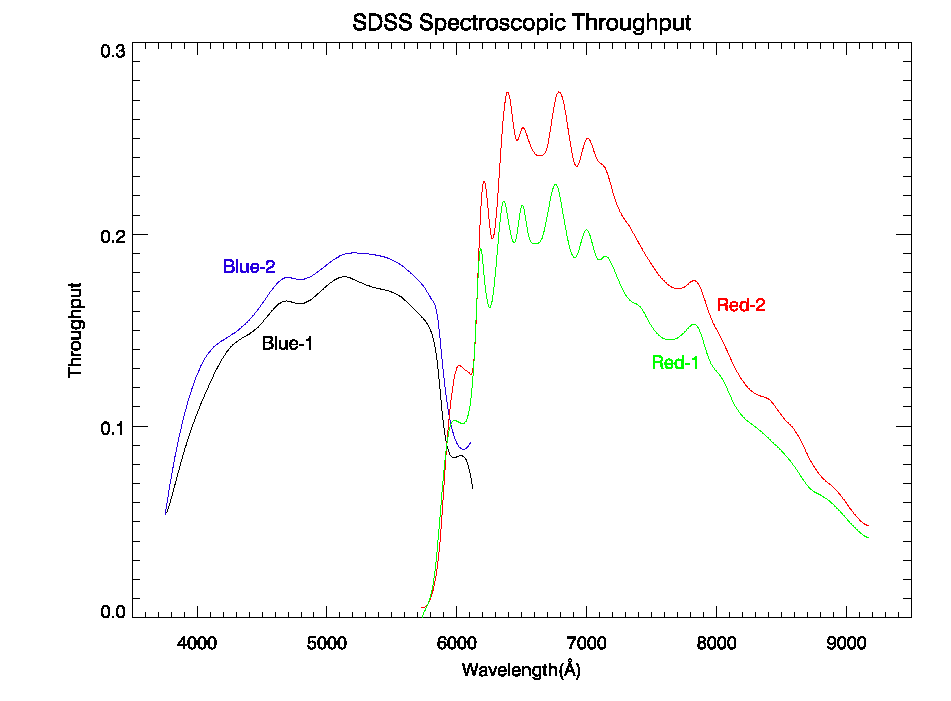
\includegraphics[angle=+90,scale=.75]{spectput.ps}

\label{fig-spectput}
\end{figure}}\hbox{}\vfil

{\newpage\clearpage\samepage
\begin{figure}\plotone{asSpline-001356-73-13.ps}

\label{fig-astromresiduals}
\end{figure}}\hbox{}\vfil

{\newpage\clearpage\samepage
\begin{figure}\includegraphics[scale=0.7]{fig_Seeing_v2.ps}


\label{fig-Seeing}
\end{figure}}\hbox{}\vfil

{\newpage\clearpage\samepage
\begin{figure}\plotone{riuzg.15.5.eps}

\label{fig-nfcalib-ghosting}
\end{figure}}\hbox{}\vfil

{\newpage\clearpage\samepage
\begin{figure}\plotone{fig_zhed.ps}

\label{fig-zhed}
\end{figure}}\hbox{}\vfil

{\newpage\clearpage\samepage
\setbox\sizebox=\hbox{$\Lambda=0.7$}\lthtmltypeout{latex2htmlSize :tex2html_wrap_inline9999: \the\ht\sizebox::\the\dp\sizebox.}\box\sizebox}\hbox{}\vfil

{\newpage\clearpage\samepage
\setbox\sizebox=\hbox{$\Omega_M=0.3$}\lthtmltypeout{latex2htmlSize :tex2html_wrap_inline10001: \the\ht\sizebox::\the\dp\sizebox.}\box\sizebox}\hbox{}\vfil

{\newpage\clearpage\samepage
\setbox\sizebox=\hbox{$H_0=100\, \rm km\,sec^{-1}\,Mpc^{-1}$}\lthtmltypeout{latex2htmlSize :tex2html_wrap_inline10003: \the\ht\sizebox::\the\dp\sizebox.}\box\sizebox}\hbox{}\vfil

\stepcounter{section}

\clearpage
\end{document}
